%
% Chapter 3
%
% Response eQTL-style paper

\chapter{Genetic architecture of transciptomic response to influenza A (H1N1)pdm09 vaccine}
\label{chap:hird_reQTL}

% TODO upreg -> increased expression

\section{Introduction}

\subsection{Genetic factors affecting influenza vaccine response}

Vaccination is the most effective way by which seasonal influenza is controlled\autocite{houser2015InfluenzaVaccinesChallenges},
and the mechanism by which influenza vaccines are efficacious is by raising strain-specific antibodies protective against future infection\autocite{nauta2009RelationshipMeanAntibody}.
% \todo{list more factors that affect flu vacc}
% \autocite{dhakal2019HostFactorsImpact}
% Growing evidences suggest that host factors including age, biological sex, pregnancy, and immune history play important roles as modifiers of influenza virus vaccine efficacy.
% We hypothesize that host genetics, the hormonal milieu, and gut microbiota contribute to host-related differences in influenza virus vaccine efficacy.
Humoral responses are influenced by vaccine-associated factors (e.g. type, dose, adjuvants), 
but are also a complex trait influenced by host genetics\autocite{mentzer2015SearchingHumanGenetic,linnik2016ImpactHostGenetic}.
Genetic variants associated with antibody response have been detected for vaccines such as hepatitis B, influenza, measles, rubella, and smallpox\autocite{linnik2016ImpactHostGenetic,dhakal2019HostFactorsImpact}.
For antibody response to seasonal influenza vaccines, studies have implicated 
genetic variation within cytokine genes, cytokine receptors\autocite{poland2008ImmunogeneticsSeasonalInfluenza};
antigen processing and intracellular trafficking genes\autocite{franco2013IntegrativeGenomicAnalysis}; 
immunoglobulin heavy-chain variable region loci\autocite{avnir2016IGHV169PolymorphismModulates};
and specific \gls{HLA} alleles \autocite{poland2008ImmunogeneticsSeasonalInfluenza,moss2013CorrelationHumanLeukocyte}.

A potential mechanism through which genetic variation can play a causal role in influenza vaccine response is through altering the expression of genes as \glspl{eQTL}.
\gls{eQTL} can have condition-specificity: an interaction between their effect on expression and different environmental contexts such as tissue or cell type\autocite{albert2015RoleRegulatoryVariation,vandiedonck2017GeneticAssociationMolecular}.
The mechanisms by which \glspl{eQTL} interact with environment are of great interest;
for example, cell type specificity can inform us about how expression is regulated in a cell type specific manner\autocite{kim-hellmuth2019CellTypeSpecific}.
In a vaccination context, an important subset of environment-interacting eQTLs are \glspl{reQTL}, defined as an eQTL whose effect interacts with external stimulation or perturbation.
reQTL have been observed in many human cell types \textit{in vitro}, or in the whole organism \textit{in vivo}.
\todo{pull in citations from intro}
As the pre- and post-stimulation environments are separated in time, a possible mechanism that leads to the observation of reQTL is a genotype-dependent change in gene expression between timepoints,
which may underly genotype-dependent differences in antibody phenotypes.

\subsection{\Glsfmtlongpl{reQTL} for seasonal influenza vaccination}

\gls{reQTL} can be mapped considering a vaccine as an \textit{in vivo} immune stimulation, looking for genotype-dependent changes in gene expression in immune cells.
Little work has been done on vaccine-stimulated reQTLs, except one study conducted for the seasonal \gls{TIV}.
\autocite{franco2013IntegrativeGenomicAnalysis} collected longitudinal data in 247 European adults:
peripheral whole blood gene expression measured at four timepoints (day 0, 1, 3, 14), 
and antibody titres measured at three timepoints (day 0, 14, 28).
They identified 20 genes with a cis-eQTL effect, expression correlation with antibody response, and either post-vaccination differential expression \emph{or} a reQTL effect at that cis-eQTL.
Genes involved in intracellular antigen transport and processing were enriched among those 20 genes.

\subsection{Chapter summary}

% NOTE: Narcolepsy controversy (more evidence for genetic interaction with Pandemrix vaccine response in particular)
The HIRD cohort represents a unique opportunity for detecting genetic contributions to influenza vaccine response.
In \autoref{ch:hird_DGE}, we observed global changes in gene expression after Pandemrix vaccination, as well as expression signatures correlated to degree of antibody response.
For seasonal influenza vaccines, the contribution is small: antibody responses in adults are largely driven by non-genetic influences such as previous influenza vaccination or infection\autocite{brodin2015VariationHumanImmune}.
\todo{distinction between expression/ab response is blurry here}
As the Pandemrix vaccine is against the pdm09 pandemic strain that was not in seasonal circulation at the time the \gls{HIRD} cohort was recruited (2010-11), 
with individuals mounting an expression response that was not recall-dominated \autocite{sobolev2016AdjuvantedInfluenzaH1N1Vaccination},
the relative contribution of genetic factors to Pandemrix response may be greater.

\todo{straighten out tenses}
In this chapter, I model the influence of common host genetic variation on longitudinal \textit{in vivo} expression response to Pandemrix.
I map cis-eQTL within each timepoint, accounting for ancestry, cell type abundance and unmeasured covariates, 
then call shared and reQTL effects from a joint model, 
looking for genes where the lead eQTL has a different effect size pre- and post-vaccination.
Many of the strongest reQTL effects involve opposite signed effects on expression for the same variant at different timepoints.
I detect a strong day 1 specific reQTL effect at \gene{ADCY3}.
Through modelling interaction of reQTL with cell type abundance estimates and statistical colocalisation with cell type specific QTL datasets, 
the reQTL signal was determined to be a monocyte-specific effect likely driven by increase monocyte abundance at day 1.
\todo{1 more sentence to round off context}

\section{Methods}

\subsection{Genotype phasing and imputation}
\label{subsec:hird_reQTL_methods_genotypePhasingAndImputation}

% 2.	Online imputation service to phase and impute chr 1-22 and X
% 2.1.	Phase with Eagle v2.4 (version in imputation logs.tar.gz)
% 2.2.	Impute with PBWT 3.1-v3.1-2-gbf6ebe2+htslib-1.3.2-199-gec1d68e-dirty (version in vcf header)
% 2.2.1.	Reference fa is human_g1k_v37.fasta (1000 genomes)
% 2.2.2.	X chrom is done in 3 chunks
% 2.2.2.1.	X:1-2699520: impute against reference resources/refs/imputation/hrc.r1.1/pbwt/HRC.r1-1.GRCh37.chrX_PAR1.shapeit3.mac5.aa.genotypes
% 2.2.2.2.	X:2699521-154931043: impute against reference resources/refs/imputation/hrc.r1.1/pbwt/HRC.r1-1.GRCh37.chrX_nonPAR.shapeit3.mac5.aa.genotypes
% 2.2.2.3.	X:154931044-155270560: impute against reference resources/refs/imputation/hrc.r1.1/pbwt/HRC.r1-1.GRCh37.chrX_PAR2.shapeit3.mac5.aa.genotypes
Prior to imputation, 213277 monomorphic variants that provide no information for imputation
Variant alleles were aligned such that the reference allele matches the GRCh37 reference, and 358 indels were removed.
Imputation for the autosomes and X chromosome was conducted using the Sanger Imputation Service, 
which involves pre-phasing with EAGLE2 (v2.4) and imputation with PBWT (v3.1) against the Haplotype Reference Consortium (r1.1) panel \url{https://www.ncbi.nlm.nih.gov/pubmed/27548312}.
% TODO: now, switch variants to SNPS. footnote no more indels
Imputed variants were lifted-over from GRCh37 to GRCh38 coordinates using CrossMap.
% 4.	Filtering
% 4.1.	BCFTOOLS_INCLUDE="MAF>$MAF_THRESH & F_MISSING<0.05 & FILTER==\"PASS\" & INFO/INFO>0.4"
% 4.2.	Use MAF thresholds 0.05, 0.10, 0.20
Poorly-imputed variants with $\text{INFO} < 0.4$ or post-imputation missingness $> 5\%$ were removed, leaving 40290981 variants.
% e.g. of more formal?
% Following standard practices, we discarded poorly imputed SNPs, defined as having an information content metric (INFO) score <0.4. We removed SNPs significantly deviated from Hardy-Weinberg equilibrium (P<1×10-10), with a call-rate ≤0.95 or minor allele frequency ≤1%, leaving 7,578,947 variants. PCA and genotype filtering were performed using the Hail framework (version 0.1).6

\subsection{Overall strategy for detecting reQTLs}
\label{subsec:hird_reQTL_overall_strategy}

Since the aim of this chapter is to identify genetic variation that affects expression response to vaccination, it may seem most direct to model the change in each individual's expression after vaccination as the response variable.
This approach has been applied for identification of condition-specific \gls{eQTL}, typically with the response taking units of log fold change between conditions (e.g. \autocite{maranville2011InteractionsGlucocorticoidTreatment,ackermann2013ImpactNaturalGenetic,shpak2014EQTLAnalysisHuman}).
Although potentially powerful if \gls{eQTL} effects are small and opposite between conditions\autocite{ackermann2013ImpactNaturalGenetic}, 
it is analogous to the \enquote{change score} approach, which can suffer from regression to the mean (??), and increased uncertainty from the variance sum law if effects between conditions have positive covariance\autocite{allison1990ChangeScoresDependent,clifton2019CorrelationBaselineScore}.
%
% Step 1: why not intra-individual change score, why not ANCOVA, why strat and diff?
% half a century of debate
% https://digscholarship.unco.edu/cgi/viewcontent.cgi?article=1239&context=dissertations
% https://ruor.uottawa.ca/bitstream/10393/35843/3/Lemay_Julien_2017_Thesis.pdf

% TODO:
% in observational: https://www.tandfonline.com/doi/abs/10.1080/00273171.2013.831743?scroll=top&needAccess=true&journalCode=hmbr20
% in RCT: senn says equiv: https://www.google.com/url?sa=t&rct=j&q=&esrc=s&source=web&cd=&ved=2ahUKEwie_PK6vsvsAhXXRRUIHdUfD_wQFjAAegQIAxAC&url=http%3A%2F%2Fimaging.mrc-cbu.cam.ac.uk%2Fstatswiki%2FFAQ%2Frt1d%3Faction%3DAttachFile%26do%3Dget%26target%3Dsenn.ppt&usg=AOvVaw0Rp28syfyesdecEiQZw9x_
% pearl says: ?
% senn in observational: ?? https://onlinelibrary.wiley.com/doi/abs/10.1002/sim.2682
%
\todo{upend change score bit, here expression is a y variable. compare all the options as glms etc.}
% TODO: Write both as special cases of glm, and highlight their different assumptions
% TODO: mention: in ch2, used residualised change score, here, different
% Our data structure is
% Over all approach is stratified
%
% 2 schools of thought. 50 years of debate
% Change score assigns special status, assumes a specific correlation
% ...
%
% Besides not even estimatejng the same effect
%
% Many other models reduce to change score
%
% Mixed is flexible, but overall aim aligns with change score
%
% Simplest application of developed eqtl methods

% joint method over interaction
%     large numbers of conditions, not practical to use interactions

% pros for split
%     limix not ok with repeated samples in kinship matrix
%     peer not directly applicable
    
% change score should ask average of individual diffs
% strat and interaction should ask diff in averages
% interaction is further borrowing info
%
% NOTE: see
% Senn: Statistical Issues in Drug Development
% 7.2.4 Is clinical relevance a relevant consideration when choosing whether to use change scores or raw outcomes as the efficacy measure?

% TODO:  
 % It is imperative to adjust for the baseline value anyway, using regression modeling (for reasons of bias reduction in observational studies and for maximizing power and precision in randomized trials).
 % Using each patient as her own control through calculation of a change score is worse than using no control if the baseline is noisy. If the correlation between baseline and follow-up measurement is less than 0.5, subtracting the baseline is worse than just analyzing the follow-up measurement.
 % http://biostat.mc.vanderbilt.edu/wiki/Main/MeasureChange

Instead, I map \glspl{eQTL} within each of three timepoint conditions (day 0 pre-vaccination, day 1, and day 7), and find \glspl{reQTL} by looking for \glspl{eQTL} that have different effects between conditions.
% TODO: would use ANCOVA here i.e. equiv to continuous covar in regression
% TODO it is not the case people act as their own controls, you can't observe the counterfactual outside of n of 1 trials
% more like soaking up some of the variation as within individual random effect, allowing more precise
% also see: https://blog.statsols.com/making-it-personal-n-of-1-trials-allowing-for-individuality-but-not-overdoing-it
\todo{Can this really demonstrate genotype-dependent change in gene expression between timepoints? i.e. need understand how the change score/ANCOVA approaches differ from repeated measures ANOVA differ from the interaction/stratified approach I take?}
Unlike a test for difference implemented using a genotype-condition interaction term in a joint regression model, homoscedasticity of errors is not assumed for all conditions\autocite{clogg1995StatisticalMethodsComparing}
% See PMC4425538 : The method we have used did not account for heteroscedasticity while estimating the standard errors of the interaction term, which may lead to inflated statistics.
% TODO: equivalence is not straightforward, since of joint mashr downstream

% real killer is missing data for manova/ancova
% TODO: also MANOVA
% Instead of just accommodating unequal variances and covariance within a subject, the mixed models approach directly models the covariance structure of the multiple dependent variables.
% https://blogs.sas.com/content/sastraining/2011/02/02/the-punchline-manova-or-a-mixed-model/
% https://stats.stackexchange.com/questions/13197/differences-between-manova-and-repeated-measures-anova
% avoids sphericity http://www.discoveringstatistics.com/docs/sphericity.pdf
%
% But, we are interested in interaction, and this is not directly answered by manova (i.e. multivariate mode in limix)

% Independence: errors assoc with one observation are not correlated with erros of any other
% Homoscedasticity: Var y does not depend on x

% Step 2: why stratification/subgroup not interaction
% TODO interaction is more efficient under certain assumptions
%     https://stats.stackexchange.com/questions/332963/why-may-results-from-model-with-interaction-term-and-stratified-model-be-differe
% These models will consistently estimate the same thing only when the mean model is true.
% possible here since time is not treated as continuous
% https://stats.stackexchange.com/questions/93540/testing-equality-of-coefficients-from-two-different-regressions
    % I found the key difference is whether the assumption that the error variance is the same or not.
% https://stats.stackexchange.com/questions/55501/test-a-significant-difference-between-two-slope-values
    % The classic (and more statistically powerful) way of testing this is to combine both datasets into a single regression model and then include the area as an interaction term. See, for example, here:
    % http://www.theanalysisfactor.com/compare-regression-coefficients/
    % This is "more ... powerful" only if more restrictive assumptions apply. In particular, it assumes homoscedasticity of error variances. Often one would not want to assume that (without additional justification) and therefore would use something like the Welch or Satterthwaite t-test. – whuber♦ Mar 30 '16 at 21:46
%
% https://stats.stackexchange.com/questions/33692/joint-model-with-interaction-terms-vs-separate-regressions-for-a-group-comparis
%     The first model will fully interact gender with all other covariates in the model. Essentially, the effect of each covariate (b2, b3... bn). In the second model, the effect of gender is only interacted with your IV. So, assuming you have more covariates than just the IV and gender, this may drive somewhat different results.
% i.e. there are interactions between time and ALL VARIABLES
%
% whereas interaction model pools estimates (borrows info)
%
% cons:
% interaction gives direct p nominal value, we have to estimate
% but how to control for multiplicity?
%
% Statistical Approaches for Estimating Sex-Specific Effects in Endocrine Disruptors Research
% https://ehp.niehs.nih.gov/doi/10.1289/EHP334 < TODO
%
% also see homo: https://cris.maastrichtuniversity.nl/ws/files/11868404/799719.pdf
% TODO:
% really, pro is Simplicity
% Can do interactions
% Can do coloc
% Can use peer
% interaction with time fixed fx vs stratified
% \todo{interactions, apart from scalability genome wide, and additional complexity when also adding cell type and platform interactions, and assumption of homoscedascity between all groups}
% vs pooling power
%
% note intent to use joint modelling later, so as to not lose info and fall into jelly bean problem https://www.ahajournals.org/doi/10.1161/CIRCULATIONAHA.108.836601

% TODO: honestly given i used change score in ch2, the biggest motivator is probably practicality e.g. ability to use PEER

%
% DEPRECATED:
% How to meta-analyse? We are restricted to non-full Bayesian methods.
%
% See last paragraph of discussion in
% Kontopantelis, E., Springate, D. A., & Reeves, D. (2013). A Re-Analysis of the Cochrane Library Data: The Dangers of Unobserved Heterogeneity in Meta-Analyses. PLoS ONE, 8(7), e69930. https://doi.org/10.1371/journal.pone.0069930
% For small k, Sidik MVa or Ruhkin RBp recommended.
%
% metafor manual
% If, instead of the crude estimate, one wants to use a better apriori estimate, one can do so by passing this value via control=list(tau2.init=value)
% Sidik-Jonkman estimator, also called the ‘model error variance estimator’, is implemented in metafor (SJ method).
% Starts with an init estiamte of ri=sigma2i/tau2i i.e. ratio of study-specific and between-studies het variance, then updates.
% They recommend using Hedges [1], to init, but this is bad???
% We use mode of gamma as an apriori estimate of tau.
%
% 2.7.	Meta-analysis with metafor
% 2.7.1.	Per day, use rma(‘REML’) to fit random-effects model on association beta and beta_ste, per gene-SNP pair, using all timepoints from array/RNA-seq for that day
% 2.8.	eigenMT to get number of independent tests per gene
% 2.8.1.	split previously generated geneloc and snpsloc by chrom
% 2.8.2.	per chrom, run eigenMT on limix output (arbitrary day, since the set of snps cis to each gene does not vary by day)
% 2.9.	Compute hierarchical FDR
% 2.9.1.	Per day
% 2.9.1.1.	Use eigenMT estimates to apply local Bonferroni per gene
% 2.9.1.2.	Compute global BH FDR
Within each timepoint, recall the the \gls{HIRD} dataset includes expression measured by both array and \gls{RNAseq}.
As discussed in \autoref{subsubsec:hird_dge_meta_methodChoice}, it is difficult to directly estimate the between-studies heterogeneity when the number of studies is small, 
and Bayesian meta-analysis was preferred for combining array and \gls{RNAseq} \gls{DGE} estimates.
\todo{why I didn't just do a mega-analysis in chapter 2 then, given I haven't any evidence if it's better or worse than Bayesian meta-analysis in that context.}
That method does not scale to \gls{eQTL} analysis, where the number of tests is large, in the order of thousands of tests per gene, versus the handful \gls{DGE} contrasts per gene performed in \autoref{ch:hird_DGE}.
Instead, I perform a mega-analysis within each timepoint, first merging array and \gls{RNAseq} expression estimates into a single matrix with ComBat\autocite{johnson2007AdjustingBatchEffects}.
For comparison purposes, analyses were also run using in the array and \gls{RNAseq} samples separately.
\todo{add -7 note as with ch2}

Defining whether an \gls{eQTL} is shared between conditions can be a tricky business.
Naively, one can map \glspl{eQTL} separately in each condition, then assess the overlap of significant associations between conditions.
This underestimates sharing due to the difficulty of distinguishing true lack of sharing from missed discoveries from incomplete power within each condition \autocite{flutre2013StatisticalFrameworkJoint,peters2016InsightGenotypePhenotypeAssociations}.
Condition-by-condition analysis also cannot borrow information across conditions for mapping shared associations\autocite{flutre2013StatisticalFrameworkJoint,urbut2018FlexibleStatisticalMethods,li2018HTeQTLIntegrativeExpression}.
Counterintuitively, a joint multivariate analysis may be more powerful even when associations are not shared across all conditions\autocite{stephens2013UnifiedFrameworkAssociation}.

% 2018-07-25 log: HIRD eQTL modelling possibilities
% General pattern of development:
% MANOVA < MetaTissue
% MetaTissue < JAGUAR < RECOV
% Metasoft < mashr
% eqtlbma < mashr
% MetaTissue < MT-eQTL < HT-eQTL
%
% Excellent history from the HT-eQTL paper https://bmcbioinformatics.biomedcentral.com/articles/10.1186/s12859-018-2088-3
% Recently, the NIH Common Fund’s Genotype-Tissue Expression (GTEx) project has undertaken a large-scale effort to collect and analyze eQTL data in multiple tissues on a growing set of human subjects, and there has been a concomitant development of methods for the analysis of such data.
% For example, Peterson et al. [3] and Bogomolov et al. [4] developed new error control procedures to control false discovery rates at different levels of resolution (e.g., at the SNP level or the gene level) for eQTL analysis.
% The methods have been used to identify genes whose expression is regulated by SNPs (eGenes), or SNPs that affect the expression levels of multiple genes (eSNPs).
% However, the methods only concern how to reduce the number of hypotheses in a hierarchical structure, but cannot effectively borrow strength across tissues to enhance eQTL discoveries.
% Lewin et al. [5], Sul et al. [6] and Han et al. [7] developed regression-based methods via Bayesian multivariate regression and random-effects models.
% The models accommodate data from multiple tissues simultaneously, and integrate information across tissues for eQTL detection.
% However, a potential drawback is that they only focus on one gene or gene-SNP pair at a time, and fail to leverage information across different gene-SNP pairs.
% Flutre et al. [8] and Li et al. [9] developed hierarchical Bayesian models to model summary statistics across multiple tissues.
% The models capture the marginal distribution of each gene-SNP pair with interpretable parameters, and explicitly characterize heterogenous eQTL configurations in multiple tissues.
% However, the model fitting is computationally expensive and cannot scale to a large number of tissues.
% Recently, Urbut et al. [10] proposed an ad hoc approach based on shrinkage to improve the scalability of the Bayesian models.
% However, the procedure is subject to overfitting and the model parameters are hard to interpret.
%
A variety of models have been employed for joint \gls{eQTL} mapping, including
the use of classical multivariate methods such as \gls{MANOVA}\autocite{kim2014CharacterizingGeneticBasis},
frequentist meta-analyses (e.g. \software{Meta-Tissue}\autocite{sul2013EffectivelyIdentifyingEQTLs}, METASOFT), 
and Bayesian models (e.g. eQtlBma\autocite{flutre2013StatisticalFrameworkJoint}, MT-HESS, MT-eQTL).
Joint mapping has been repeatedly been demonstrated to be more powerful than condition-by-condition analysis,
and recent methods are now computationally efficient when scaling to large numbers of conditions and variants tested (e.g. RECOV\autocite{duong2017ApplyingMetaanalysisGenotypetissue}, mashr\autocite{urbut2018FlexibleStatisticalMethods}, HT-eQTL\autocite{li2018HTeQTLIntegrativeExpression}).
In this chapter, I apply \software{mashr}\autocite{urbut2018FlexibleStatisticalMethods} for the estimation of \gls{eQTL} effects across my three timepoints.
\software{mashr} learns patterns of correlation among multiple conditions empirically from condition-by-condition summary statistics,
then applies shrinkage to provide improved posterior effect size estimates,
and compute measures of significance per condition. 

% TODO
% mashr: build on traditional metaanalysis methodology (see urbut)

\subsection{Controlling for population structure with \glsfmtlongpl{LMM}}

There is population structure due to ancestry in the \gls{HIRD} cohort,
which was incorporated in \gls{DGE} analyses by treating the top \glspl{PC} of the genotype matrix as continuous covariates for large-scale population structure (\autoref{subsec:hird_dge_genotype_pc}).
In the context of \gls{eQTL} mapping (and genetic association studies in general), 
where the aim is to assess the marginal effect of a single genetic variant on expression, 
population structure can be correlated with both expression (e.g. through polygenic effects)
and the tested variant (e.g. through ancestry-dependent frequency differences).
% While genetics is more resistant to confounding due to randomisation of alleles, one of the things that can affect is ...
This leads to \gls{OVB} from confounding, which if not controlled for, leads to genome-wide inflation of test statistics \autocite{price2010NewApproachesPopulation}.
% TODO \url{https://www.nature.com/articles/srep06874}
\todo{add some indication of how much inflation can be reduced by LMMs}
% This is great background/intuition: golan2018MixedModelsCaseControl
% using LMMs is appropriate for controlling for population structure (which is a common
% problem in human GWAS), as well as for cryptic relatedness, and that LMMs outperform
% the previously preferred principal component analysis (PCA) approach in addressing these
% issues (Yang et al., 2014).
%
% Also see: 2018-11-26 notes in log
% TODO: read this Deconstructing the sources of genotype-phenotype associations in humans
An useful approach is the \gls{LMM} with a random effect that incorporates genetic correlation between individuals, usually in the form of a kinship matrix, into the covariance of that random effect\autocite{price2010NewApproachesPopulation, eu-ahsunthornwattana2014ComparisonMethodsAccount, golan2018MixedModelsCaseControl}
The \gls{LMM} approach has the advantage of not only modelling large-scale population structure, but also cryptic relatedness (the presence of closely related individuals in a sample assumed to consist of unrelated individuals\autocite{astle2009PopulationStructureCryptic}) due to finer-scale effects such as family structure\autocite{golan2018MixedModelsCaseControl}.
%
% TODO although: https://twitter.com/A_A_Zaidi/status/1285578961356034049
% When structure has a recent origin, PCA or LMMs won't fully correct for stratification if the GRM is derived from common variants as they are older and not very informative about recent demographic history.
% TODO:
% We demonstrate that widely used approaches to adjust for population structure, including principal components analysis and mixed modelling with a random effect for a genetic relationship matrix, cannot fully account for the fine-scale geographical confounding in the UK Biobank.
% fine scale: https://academic.oup.com/hmg/article-abstract/doi/10.1093/hmg/ddaa157/5874041

\subsubsection{Estimation of kinship matrices}
\label{subsec:hird_reQTL_LDAK}

% 1.	Build GRM using LDAK 5
% 1.1.	Start with pre-imputed genotypes coreex_eQTLflu_20171204.gencall.smajor.impute_sex.qc6
% 1.1.1.	“Estimates of SNP heritability are very sensitive to genotyping errors”, so we can’t use imputed SNPs without filtering for high INFO.
% 1.2.	Prune to MAF 0.05, autosomes only
% 1.3.	Compute LDAK SNP weightings
% 1.4.	Compute kinships for each chromosome
% 1.5.	Join per-chromosome kinships into genome-wide kinships
% 1.5.1.	Use the leave-one-chromosome-out strategy
%
When testing a variant for association using \glspl{LMM}, to avoid loss of power from \enquote{proximal contamination}, the kinship matrix used should not include that variant\autocite{listgarten2012ImprovedLinearMixed}.
A simple way to avoid this is to compute a \gls{LOCO} kinship matrix using all variants on chromosomes other than the tested variant's chromosome\autocite{lippert2011FaSTLinearMixed}.

I estimated kinship in the \gls{HIRD} data from common autosomal variants, using \software{LDAK} (5.0), which computes kinship matrices adjusted for bias caused by \gls{LD}\autocite{speed2012ImprovedHeritabilityEstimation}.
Filtered, pre-imputation sample genotypes from \autoref{subsec:hird_reQTL_methods_genotypePhasingAndImputation} were pruned to $\text{\gls{MAF}} > 0.05$.
A kinship matrix was computed for each autosome, then combined into a single genome-wide matrix using \software{LDAK -{}-join-kins}.
To obtain a \gls{LOCO} kinship matrix for each autosome, each autosome's kinship matrix was then subtracted from this genome-wide matrix (\software{LDAK -{}-sub-grm}).
\todo{add chr1 loco kinship matrix as example, note the estimates for self-relatedness on the diagonals are not constrained to be 1}

% Full notes about cell type correction pipeline rationale at 2019-10-30 in log

\subsection{Additional \glsfmtshort{eQTL}-specific expression preprocessing}

There are a number of transformations often applied to expression data before \gls{eQTL} mapping, 
such as the rank-based \gls{INT} (e.g. GTEx v8\autocite{aguet2019GTExConsortiumAtlas}),
which conforms often non-normal expression data to an approximately normal distribution, and reduces the impact of expression outliers.
% TODO: read https://onlinelibrary.wiley.com/doi/full/10.1111/biom.13214
In the context of genetic association studies, the practice of applying rank-based \gls{INT} to phenotypes has been criticised for only guaranteeing approximate normality of residuals when effect sizes are small,
and potential inflation of type I error, especially in linear models that include interactions\autocite{beasley2009RankBasedInverseNormal}.
In multi-condition datasets, these transformations are also typically applied within conditions (e.g. within each tissue individually in GTEx v8\autocite{aguet2019GTExConsortiumAtlas}).
% \url{https://github.com/molgenis/systemsgenetics/wiki/eQTL-mapping-analysis-cookbook-for-RNA-seq-data}
Another common transform is standardising (centering and scaling to zero mean and unit variance) (e.g. eQTLGen Consortium\autocite{vosa2018UnravelingPolygenicArchitecture}),
often done so that effects across genes and studies can be comparably interpreted in units of standard deviation expression\autocite{qi2018IdentifyingGeneTargets}.
\todo{helps with coloc}

\todo{emph here that the sims match what my def of reqtl is for rest of chapter}

I performed simulations to evaluate the effect of these transformations on reQTL detection between a hypothetical baseline and day 1 post-vaccination condition.
Expression values on the log scale were simulated with the \gls{eQTL} slope (beta) set to specific values corresponding to six scenarios for six gene-variant pairs (\autoref{fig:hird_eQTL_expressionTransform_sims}).
\todo{log scale: as interactions depend on the scale at which departure from additivity is detected}
The simulated scenarios were subjected to rank-based \gls{INT} (Blom method\autocite{beasley2009RankBasedInverseNormal}), standardisation (both centering and scaling), scaling-only, and centering-only transformations.
Transformations were applied both within each condition and without separating conditions.
% TODO: add existing papers that use mash on rank int

The boxed facets in \autoref{fig:hird_eQTL_expressionTransform_sims} represent undesirable effects of transformations on \gls{reQTL} calls.
For example, rank-based \gls{INT} induces false shared \gls{eQTL} effects in scenarios 4 and 5.
In general, transformations that scale within condition are not appropriate, as different variance between conditions can be what drives a \gls{reQTL} effect.
Scaling without separating conditions can also be problematic, since the total variance also contributes to the \gls{reQTL} effect size.
For example, scenarios 2 and 4 have the same 1 unit increase in slope pre-transformation (the same fold-change between conditions), 
but after scaling-only the beta increases are $0.75-0=0.75$ and $0.8-0.4=0.4$ respectively---eQTL 4 now looks like a weaker effect.
% TODO: this is ofc due to my definition

In light of these simulations, I decided that neither rank-based \gls{INT} nor standardisation were appropriate given my intent of detecting \glspl{reQTL} between conditions.
Only the centering-only transformation avoided both false shared effects and preserves relative \gls{reQTL} effect sizes between genes.
The simple inclusion of an intercept term in the \gls{eQTL} model already achieves this.
Not performing any rank-based transform does lose the advantage of reining in outliers.
The expression data have already been preprocessed to remove low-expression outliers in \autoref{subsec:hird_dge_rnaseq_quantAndFilter}, 
% TODO: note for a large number of samples
but automatic outlier exclusion based on \gls{SD} thresholds at the \gls{eQTL} mapping step could be considered in future implementations\autocite{vosa2018UnravelingPolygenicArchitecture}.
Note that many preprocessing steps done prior to this stage in the pipeline (e.g. variance-stabilisation, ComBat batch effect correction) are also expression transformations,
but I only consider the preservation of \gls{reQTL} effects defined from expression values post-adjustment for those technical effects to be important.

% TODO: https://github.com/eliocamp/tagger/issues
\begin{figure}
    \centering
    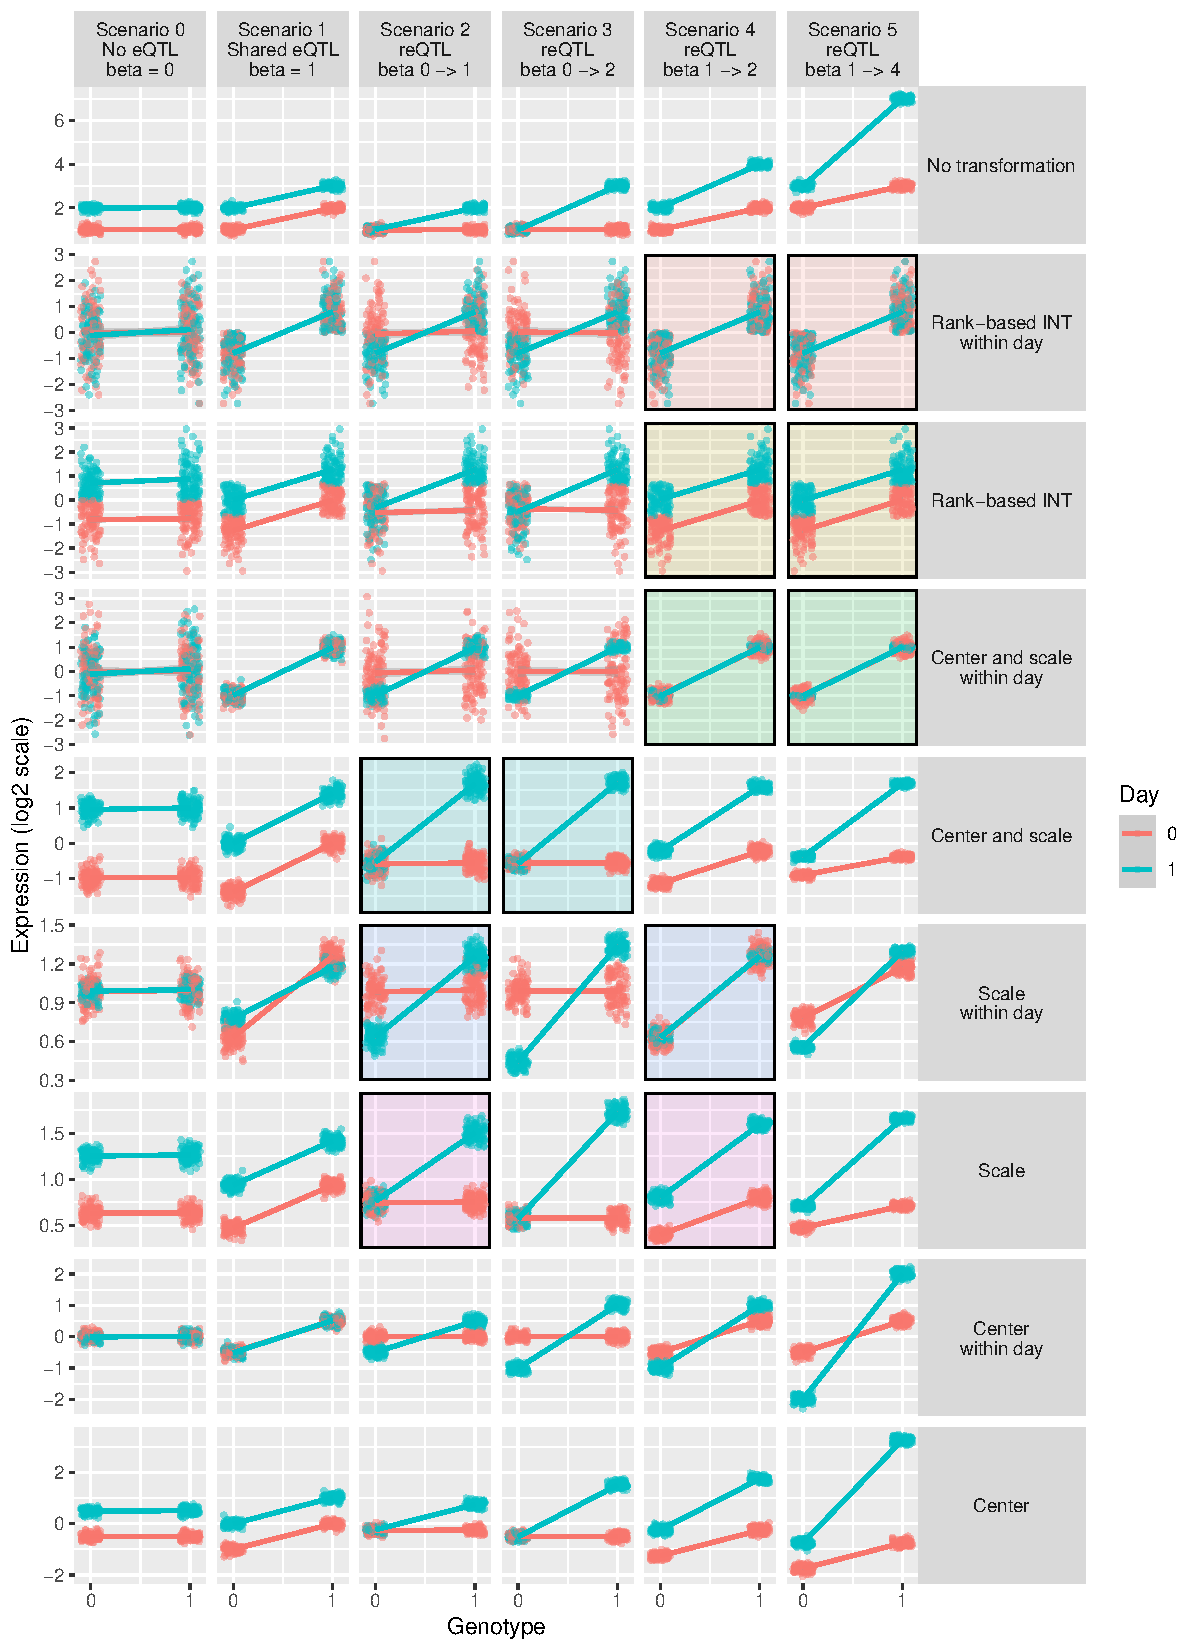
\includegraphics[width=1.0\textwidth,page=1]{mainmatter/figures/chapter_03/simulate_expression_transforms.pdf}
    \caption{
        Simulated log scale expression in two conditions for six genes (columns) representing six different scenarios:
            Scenario 0 has no \gls{eQTL}, 
            scenario 1 is a shared eQTL (beta = 1), 
            scenario 2 is a \gls{reQTL} where beta increases from 0 to 1,
            scenario 3 is a \gls{reQTL} where beta increases from 0 to 2,
            scenario 4 is a \gls{reQTL} where beta increases from 1 to 2,
            and scenario 6 is a \gls{reQTL} where beta increases from 1 to 4.
            Rows represent the effect of different expression transformations across samples, conducted both within condition, and including both conditions.
    }
    \label{fig:hird_eQTL_expressionTransform_sims}
\end{figure}
\todo{add sample sizes and model for expression sim}

\subsection{Estimation of cell type abundance from expression}
\label{subsec:hird_reQTL_xCell}

\Gls{PBMC} samples are a mixture of immune cells, and a fixed input of RNA extracted from that mixture is used to estimate expression, 
so estimates for genes that have cell type specific expression depend on the relative proportions of each cell type in each sample.
These proportions shift after Pandemrix vaccination\autocite{sobolev2016AdjuvantedInfluenzaH1N1Vaccination},
and \gls{eQTL} effects can also be cell type specific\todo{determine appropriate citations from existing refs in intro}.
As genotype can be assumed to stay constant, it is valid to compare the effect of genotype on expression between multiple timepoints to call \glspl{reQTL}, 
but changes in cell type abundance influence this by \todo{??} both expression and the effect of genotype on expression.
% TODO: https://journals.lww.com/epidem/Fulltext/2009/11000/On_the_Distinction_Between_Interaction_and_Effect.16.aspx
Immune cell abundance also varies naturally between healthy individuals\autocite{brodin2015VariationHumanImmune,brodin2017HumanImmuneSystem}, so it is important to model these effects even at baseline.

Cell type abundance directly measured via \gls{FACS} are only available for a small subset of \gls{HIRD} individuals (\autoref{subsec:hird_dge_studyDesign}), so I derived cell type abundance estimates from the expression data as an alternative.
Such estimates have previously been used in \gls{eQTL} analyses from bulk samples where cell type specific effects are expected\autocite{westra2015CellSpecificEQTL,davenport2018DiscoveringVivoCytokineeQTL,kim-hellmuth2019CellTypeSpecific}.
As the estimates are based on the expression of multiple genes, is not entirely circular to use them as covariates in this way for genewise \gls{eQTL} models.
% https://github.com/dviraran/xCell
%
% xCell uses the expression levels ranking and not the actual values, thus
% normalization does not have an effect, however normalizing to gene length is
% required.
%
% Importantly, xCell performs best with heterogenous dataset. Thus it is
% recommended to use all data combined in one run, and not break down to pieces
% (especially not cases and control in different runs).  xCell uses the
% variability among the samples for the linear transformation. xCell will only
% function with heterogenous mixtures. If there is no variability between the
% samples, xCell will not identify any signal. As noted above, it is highly
% recommended to use all data combined in one run. Failing to do so will again
% inevitably make xCell's results false.
%
% xCell produces enrichment scores, not percentages. It is not a deconvolution
% method, but an enrichment method. That means that the main usage is for
% comparing across samples, not across cell types. xCell does an attempt to make
% the scores resemble percentages, but it is a hard problem, and is very platform
% and experiment specific. We have made some tests to compare the ability of
% xCell for cross-cell types analysis, and found that it generally performed
% better in that than other methods (on limited and comparable cell types), but
% this type of analysis should be performed carefully.  Regarding this issue,
% scaling the scores by samples is extremely dangerous and will inevitably will
% result in false interpretations.
I selected \software{xCell}\autocite{aran2017XCellDigitallyPortraying}, which previously been shown to outperform other deconvolution methods for cell type specific \gls{eQTL} mapping in blood\autocite{kim-hellmuth2019CellTypeSpecific}.
\software{xCell} computes enrichment scores based on the expression ranks of approximately 10000 signature genes derived from purified cell types,
works for both array and \gls{RNAseq} expression data,
and implements \enquote{spillover compensation} to reduce dependency of estimates between related cell types\autocite{aran2017XCellDigitallyPortraying}.
%
% The spillover compensation step may over compensate, thus it is always better
% to run xCell with a list of cell types that are expected to be in the mixture.
% The names of cell types in this list must be a subset of the cell types that
% are inferred by xCell.
%
\software{xCell} was originally developed for tumor samples, so many of the built-in cell types are not expected in \gls{PBMC}.
% See 2019-11-14 log
% https://link.springer.com/chapter/10.1007/978-3-319-16104-4_15
% https://www.nature.com/articles/s41588-018-0089-9
% www.blueprint-epigenome.eu/index.cfm?p=7BCEDA45-EC73-3496-2C823D929DD423DB
Reviewing the literature to find which broad classes of peripheral blood cell types are commonly-expected in the \gls{PBMC} compartment\autocite{kleiveland2015PeripheralBloodMononuclear,vanderwijst2018SinglecellRNASequencing,davenport2018DiscoveringVivoCytokineeQTL},
I selected 7/64 of the built-in cell types: CD4\textsuperscript{+} T cells, CD8\textsuperscript{+} T cells, B cells, plasma cells, \gls{NK} cells, monocytes, and \glspl{DC}.
% /nfs/users/nfs_b/bb9/workspace/phd/output/hird/rnaseq/4_de/array/array_data_setup.y.filtered.MaxMean.combat.rds
% and /nfs/users/nfs_b/bb9/workspace/phd/output/hird/rnaseq/4_de/array/array_data_setup.sample.metadata.merged.rds
Array and \gls{RNAseq} data from \autoref{subsec:hird_dge_array_preproc} and \autoref{subsec:hird_dge_rnaseq_quantAndFilter} were processed through \software{xCell} separately.
The large batch effect present in the array expression was first removed using ComBat.
Finally, enrichment scores were standardised, so that a score of zero estimates the average abundance of that cell type across all timepoints (\autoref{fig:hird_xCell_scores_heatmap_array} and \autoref{fig:hird_xCell_scores_heatmap_rnaseq}).
\todo{add comment on existence of chosen cell types in samples, and clustering by visit}

\begin{figure}
    \centering
    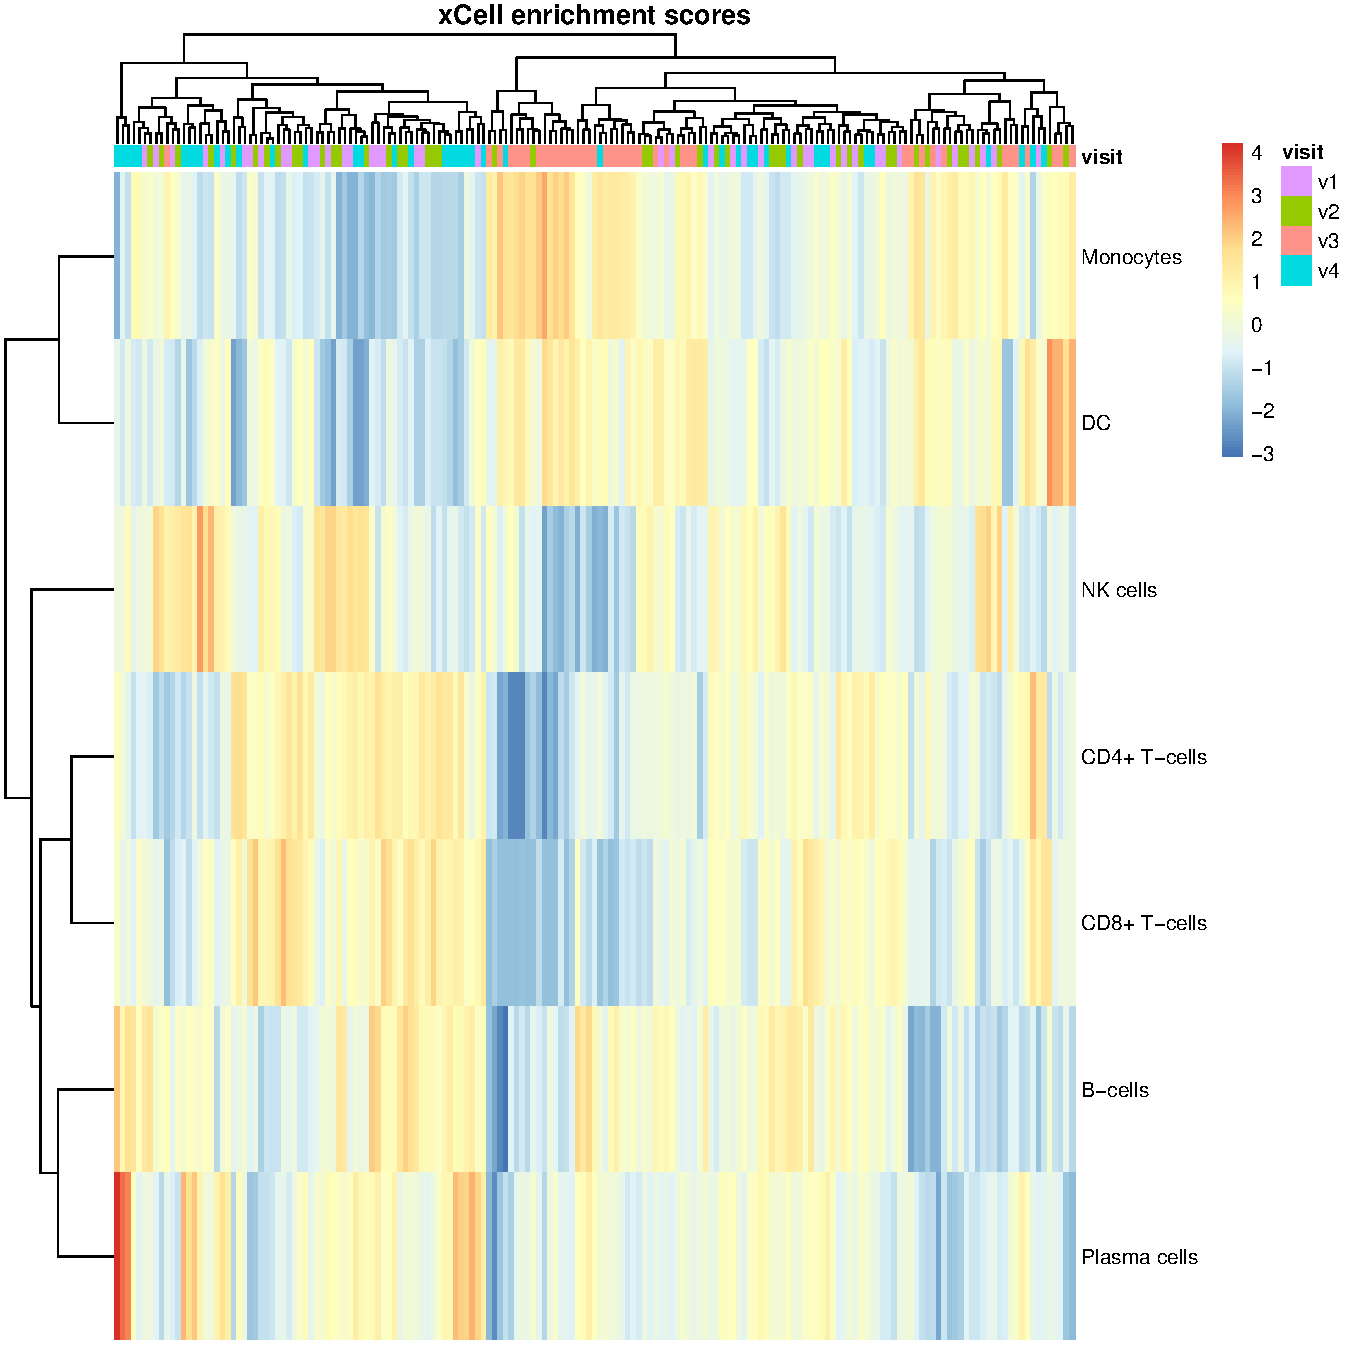
\includegraphics[width=1.0\textwidth,page=1]{mainmatter/figures/chapter_03/get_xCell_estimates.dataset_array.plots.pdf}
    \caption{Standardised xCell enrichment scores for seven \gls{PBMC} cell types in array samples.}
    \label{fig:hird_xCell_scores_heatmap_array}
\end{figure}

\begin{figure}
    \centering
    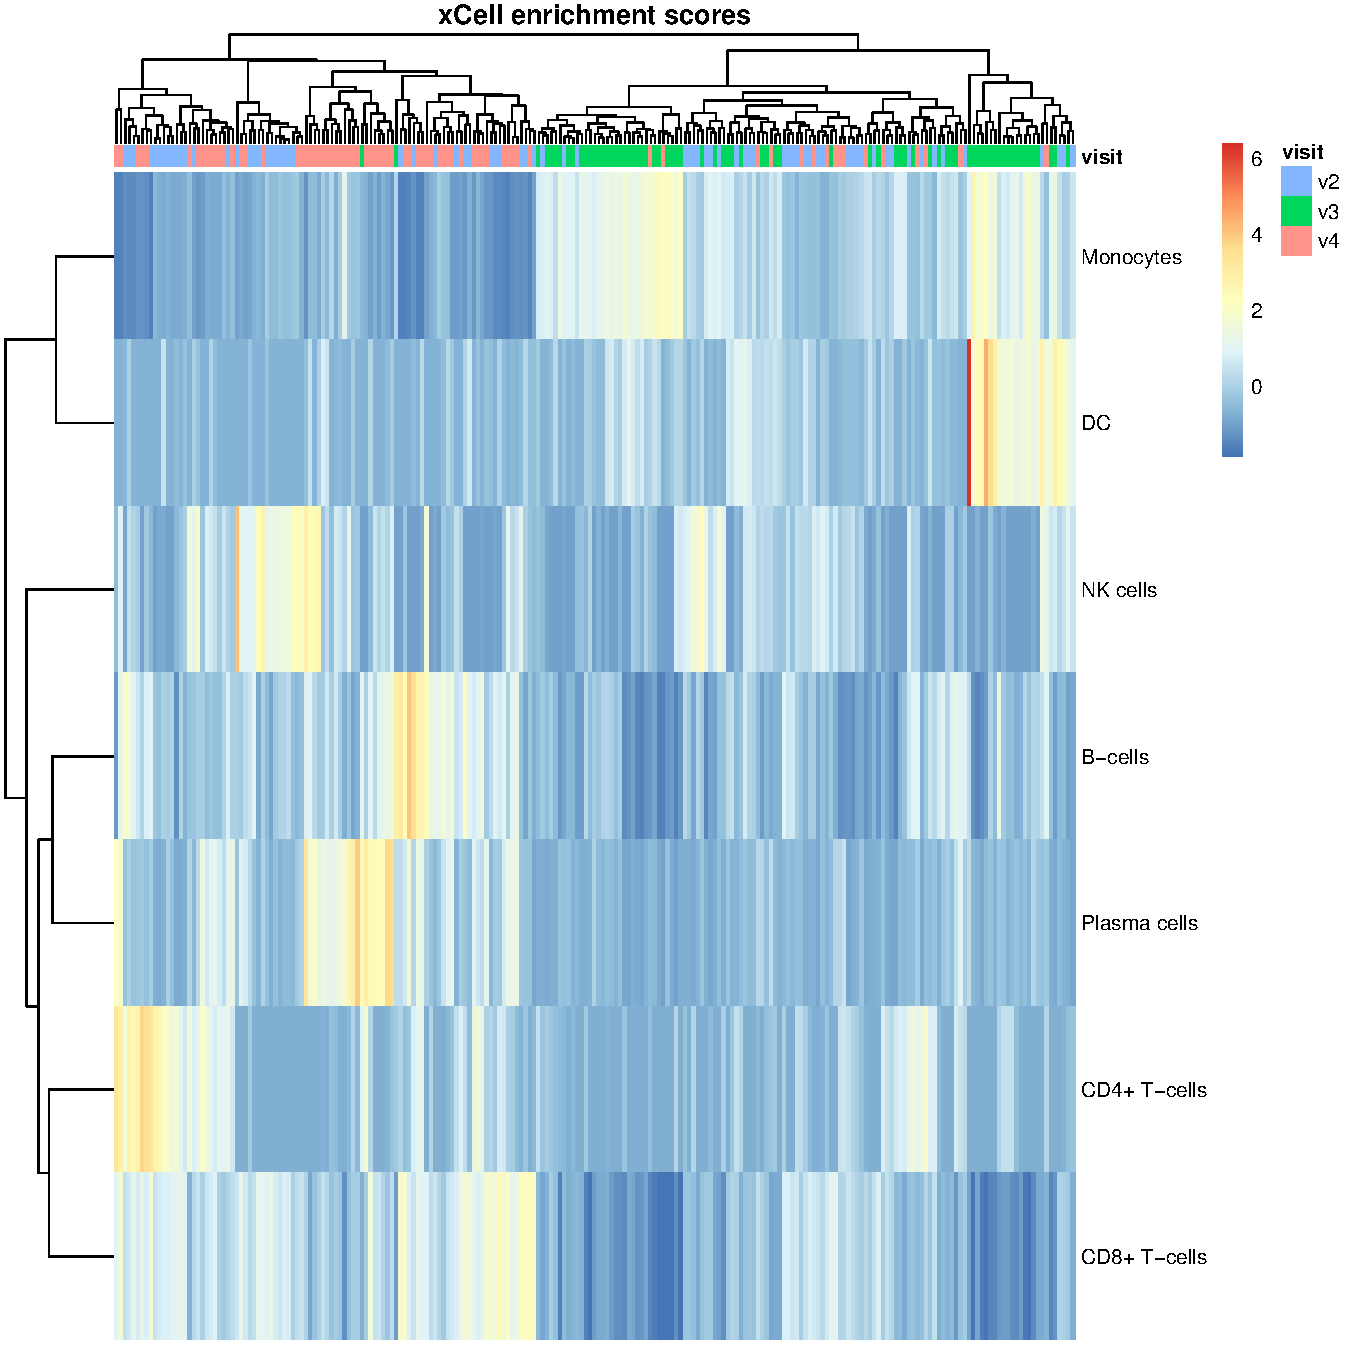
\includegraphics[width=1.0\textwidth,page=1]{mainmatter/figures/chapter_03/get_xCell_estimates.dataset_rnaseq.plots.pdf}
    \caption{Standardised xCell enrichment scores for seven \gls{PBMC} cell types in \gls{RNAseq} samples.}
    \label{fig:hird_xCell_scores_heatmap_rnaseq}
\end{figure}

As with actual cell type abundances, the enrichment scores are correlated.
Multicollinearity will be a problem for interpreting effect size estimates when these scores are used as indepedent variables in regression downstream.
% TODO not the sizes
\todo{does not bias least squares regression, but unstable (vary sample to sample) to changes in data due to sampling var, and more std error of estimates will be high (tending to inf if perfect multi)}
\footnote{high intercorrelation is not necessary nor sufficient by itself to induce multicollinearity, but multiple correlation does have an inverse relationship with the standard error of coefficient estimates \autocite{maddala1992IntroductionEconometrics}}
To prune the number of scores, I performed a \gls{PCA} of the cell type scores across samples,
% Kaiser Rule
% The more variables that load onto a particular component (i.e., have a high
% correlation with the component), the more important the factor is in
% summarizing the data. An eigenvalue is an index that indicates how good a
% component is as a summary of the data. An eigenvalue of 1.0 means that the
% factor contains the same amount of information as a single variable. [note 1]
determined the number of principal components that exceed the eigenvalues-greater-than-one rule of thumb\autocite{kanyongo2005InfluenceReliabilityFour},
then selected only the one cell type with the highest contribution for each of those components.
In both array and \gls{RNAseq} datasets, the number of components retained was three, and the selected cell types were monocytes, \gls{NK} cells, and plasma cells (\autoref{fig:hird_xCell_cos2}).
The choice to use the actual cell type scores over principal components directly as covariates is a sacrifice of orthogonality for interpretability.
% TODO: add percent var explained by the 3

% var$contrib: contains the contributions (in percentage) of the variables to the
% principal components. The contribution of a variable (var) to a given principal
% component is (in percentage) : (var.cos2 * 100) / (total cos2 of the
% component).
% TODO missing scree plot in array file
\begin{figure}
    \centering
    \begin{subfigure}[b]{1.0\textwidth}
        \centering
        \includegraphics[width=1.0\textwidth,page=8]{mainmatter/figures/chapter_03/get_xCell_estimates.dataset_array.plots.pdf}
        \caption{Array estimates.}
    \end{subfigure}%
    \vspace{1em}\vfill%
    \begin{subfigure}[b]{1.0\textwidth}
        \centering
        \includegraphics[width=1.0\textwidth,page=9]{mainmatter/figures/chapter_03/get_xCell_estimates.dataset_rnaseq.plots.pdf}
        \caption{\gls{RNAseq} estimates.}
    \end{subfigure}%
    \caption{Quality of representation (cos2) for each input variable in each \gls{PC} dimension after \gls{PCA} of xCell scores. Higher cos2 represents higher contribution of that variable to that dimension.}
    \label{fig:hird_xCell_cos2}
\end{figure}
\todo{no need for both size and color, use one for contribution percent}

Scores were validated against \gls{FACS} measurements in the subset of individuals that had them.
\todo{add info on the markers used for the chosen FACS counterparts}
Depending on each panel's gating strategy for each cell subset, the \gls{FACS} data were in units of either absolute counts, or percentage of the previously gated population.
A rank-based \gls{INT} was applied within each panel and cell subset, so that the transformed measure could be compared between individuals for each subset (\autocite{astle2016AllelicLandscapeHuman} takes a similar approach for cell abundance data using a quantile-based \gls{INT}).
% RANK INT also used in phenome scan PHEASANT https://www.biorxiv.org/content/biorxiv/early/2017/02/26/111500.full.pdf
%
% missForest is a nonparametric imputation method for basically any kind of data.
% It can cope with mixed-type of variables, nonlinear relations, complex
% interactions and high dimensionality(p>>n). It only requires the observation
% (i.e. the rows of the data frame supplied to the function) to be pairwise independent.
Missing values were imputed with \software{missForest}, a random forest imputation method suitable for high-dimensional data where $p \gg n$.
% NOTE:
% Why impute for cell counts but not for expression data?
% - expression matrices are mostly complete, and we only exclude genes based on low expression in RNAseq
% - we cannot drop whole FACS panels so easily like we can drop genes
Although the increase in xCell score for monocytes at day 1 and plasma cells at day 7 reflect the increases in these cell types observed by\autocite{sobolev2016AdjuvantedInfluenzaH1N1Vaccination}, overall correlation between xCell and \gls{FACS} was weak (\autoref{fig:hird_xCell_vs_FACS}).
Weighing the downside of having imperfect estimates of cell type abundance against the downsides of not accounting for abundance, or excluding samples without \gls{FACS} measures, I chose to continue the analysis using the xCell scores.

\begin{figure}
    \centering
    \begin{subfigure}[b]{0.43\textwidth}
        \centering
        \includegraphics[width=1.0\textwidth,page=6]{mainmatter/figures/chapter_03/validate_xCell_estimates.cell_type_pairs.pdf}
        \caption{Monocytes.}
    \end{subfigure}%
    \vspace{1em}\vfill%
    \begin{subfigure}[b]{0.43\textwidth}
        \centering
        \includegraphics[width=1.0\textwidth,page=3]{mainmatter/figures/chapter_03/validate_xCell_estimates.cell_type_pairs.pdf}
        \caption{\gls{NK} cells.}
    \end{subfigure}%
    \vspace{1em}\vfill%
    \begin{subfigure}[b]{0.43\textwidth}
        \centering
        \includegraphics[width=1.0\textwidth,page=2]{mainmatter/figures/chapter_03/validate_xCell_estimates.cell_type_pairs.pdf}
        \caption{Plasma cells.}
    \end{subfigure}%
    \caption{Correlation between standarised xCell scores and normalised \gls{FACS} measurements for a similar immune subset, in the subset of individuals with \gls{FACS} data.}
    \label{fig:hird_xCell_vs_FACS}
\end{figure}
\todo{get subset size}
\todo{change corr scatterplots to corr matrix}

\subsection{Finding hidden covariates using factor analysis}

% If RANKINT, why RANKINT before PEER?
%
% Are your covariates under control? How normalization can re-introduce covariate effects
% https://www.ncbi.nlm.nih.gov/pubmed/29706643
% "Many statistical tests rely on the assumption that the residuals of a model are normally distributed [1]. In genetic analyses of complex traits, the normality of residuals is largely determined by the normality of the dependent variable (phenotype) due to the very small effect size of individual genetic variants [2]. However, many traits do not follow a normal distribution."
% "applying rank-based INT to the dependent variable residuals after regressing out covariates re-introduces a linear correlation between the dependent variable and covariates, increasing type-I errors and reducing power."

% 2.	Infer global confounders by detecting hidden factors affecting expression with PEER
% 2.1.	“batch effects and other global confounders reduce the power to find expression quantitative trait loci”
% 2.1.1.	“We assume that these variables have a broad influence, and thus each of them has an effect size for every gene.”
% 2.1.2.	“The learned variables can be constrained to affect known sets of genes via a prior connectivity matrix. By default, with no prior connectivity given, they are assumed to be global and to affect large fractions of all genes“
% 2.1.3.	Note that due to this assumption: “If large trans hotspots are dominating, associations may get erroneously explained away as confounding factors”
% 2.2.	Round input expression to integer counts
% 2.2.1.	Input is y: the scaledTPM (TPM's scaled up to library size) from tximport.
% 2.3.	Normalise for library size and variance stabilize with varianceStabilizingTransformation from DESeq2 (recommended in PEER paper)
% 2.3.1.	Vst is like a souped up log: “In all cases, the transformation is scaled such that for large counts, it becomes asymptotically (for large values) equal to the logarithm to base 2 of normalized counts.”
% 2.3.2.	Note we cannot use voom-ed expressions from the DGE pipeline, as there are some samples missing due to lack of Ab titre data
% 2.3.3.	Do not blind the transformation to experimental design matrix: “If many of genes have large differences in counts due to the experimental design, it is important to set blind=FALSE for downstream analysis.”
% 2.3.4.	Here we use a simple design matrix of groups defined by all combos of day x R/NR
% 2.4.	Run PEER by timepoint
% 2.4.1.	Match GTeX pipeline: https://github.com/broadinstitute/gtex-pipeline/tree/63b13b8ced25cf8ab8e7a26f40a495e523630a9b/qtl , with some modifications.
% 2.4.1.1.	Note this pipeline uses quantile normalized, rank INT transformed expression, as PEER input
% 2.4.2.	Quantile normalize the samples with preprocessCore::normalize.quantiles
% 2.4.2.1.	Causes the expressions of the samples to have the same empirical distribution
% 2.4.2.2.	i.e. the the highest expression in each sample is set to the mean of the highest values of all samples, and in the case of no tied values, each sample’s expressions becomes a permutation of each other sample’s
% 2.4.3.	Standardize expression of each gene with Rank-Based Inverse Normal Transformation
% 2.4.3.1.	i.e. rank the expressions of a gene, then replace with values from the standard normal e.g. > rank.based.INT(1:5, c=3/8): [1] -1.1797611 -0.4972006  0.0000000  0.4972006  1.1797611
% 2.4.4.	Setup and run PEER
% 2.4.4.1.	Allow up to 10k iterations, start with n.samples/4 PEER factors
% 2.4.4.2.	One can include known covariates. We don’t, as it causes weird things like PEER factors not being sorted in descending relevance
% 2.4.4.2.1.	~ 1 + batch + rna.conc + Gender + Age.at.vaccination..years. + PC1.imputed + PC2.imputed + PC3.imputed + PC4.imputed
% 2.4.4.2.2.	Note this includes an intercept that represents the mean expression
%
% Also interesting:
% PANAMA/LIMMI, by PEER authors
% Detecting regulatory gene–environment interactions with unmeasured environmental factors
%
Apart from cell type abundance, a myriad of other unmeasured variables contribute to expression variation.
Hidden determinants of expression variation were learnt using \software{PEER}\autocite{stegle2012UsingProbabilisticEstimation}.
As suggested by \autocite{stegle2012UsingProbabilisticEstimation}, between-sample normalisation and variance stabilisation on \gls{RNAseq} count data was performed using \software{DESeq2::vst}.
ComBat was applied to first merge array and \gls{RNAseq} data into a single log scale expression matrix per timepoint, treating the largest global effects on expression---the two array batches and three \gls{RNAseq} library prep pools (\autoref{fig:hird_expression_pcs})---as known batch effects.
% (e.g., by introducing principal components of the genotype data), is not included in the model, and it may be recapitulated in the inferred factors.
Given selected known covariates (intercept, sex, four genotype \glspl{PC} from \autoref{subsec:hird_dge_genotype_pc} representing ancestry, and the three xCell scores estimated above),
% TODO: sole motivation here is efficiency. not so much confounding. PEER finds factors that explain var. so given factors are included for the sake of downstream modelling interest
% this is also the primary motivation behind recommendation of including prognostic covariates in RCTs \url{https://trialsjournal.biomedcentral.com/articles/10.1186/1745-6215-15-139}
PEER was used to estimate additional hidden factors that explain variation in expression matrix.
Factors are assumed to be unmeasured covariates that have global effects on a large fraction of genes, 
whereas a cis-\gls{eQTL} will typically only have local effects, so including factors as covariates should not introduce dependence with the genotype term,
but should soak up some of residual variation, improving power to detect cis-\glspl{eQTL}.
The analysis was run per timepoint, otherwise global changes in expression between timepoints induced by the vaccine would be recapitulated as factors.
% TODO: not like PCs: not orthogonal or uncorrelated
% TODO: add auto relevance ,
% TODO: do not keep explaining more var. var of factors themselves declines
% and no guarantee of decreasing order when known

Correlating the estimated factors to a larger set of known covariates reveals many correlations with xCell estimates, indicating that cell type abundance does indeed have substantial global effects on the expression matrix.
There is little correlation with known array or \gls{RNAseq} batch effects, indicating ComBat did an adequate job of removing batch- and platform-dependent global effects on expression (\autoref{fig:hird_peer_corMatrix_v2_mega}).
Note that I did not leave this adjustment for PEER to perform, as ComBat estimates centering and scaling factors per gene to adjust for batch effects, whereas the use of PEER factors represent a mean-only adjustment
Given the severity of the batch effect in this dataset, especially between platforms, mean-only adjustment may be insufficient\autocite{zhang2018AlternativeEmpiricalBayes}.

\begin{figure}
    \centering
    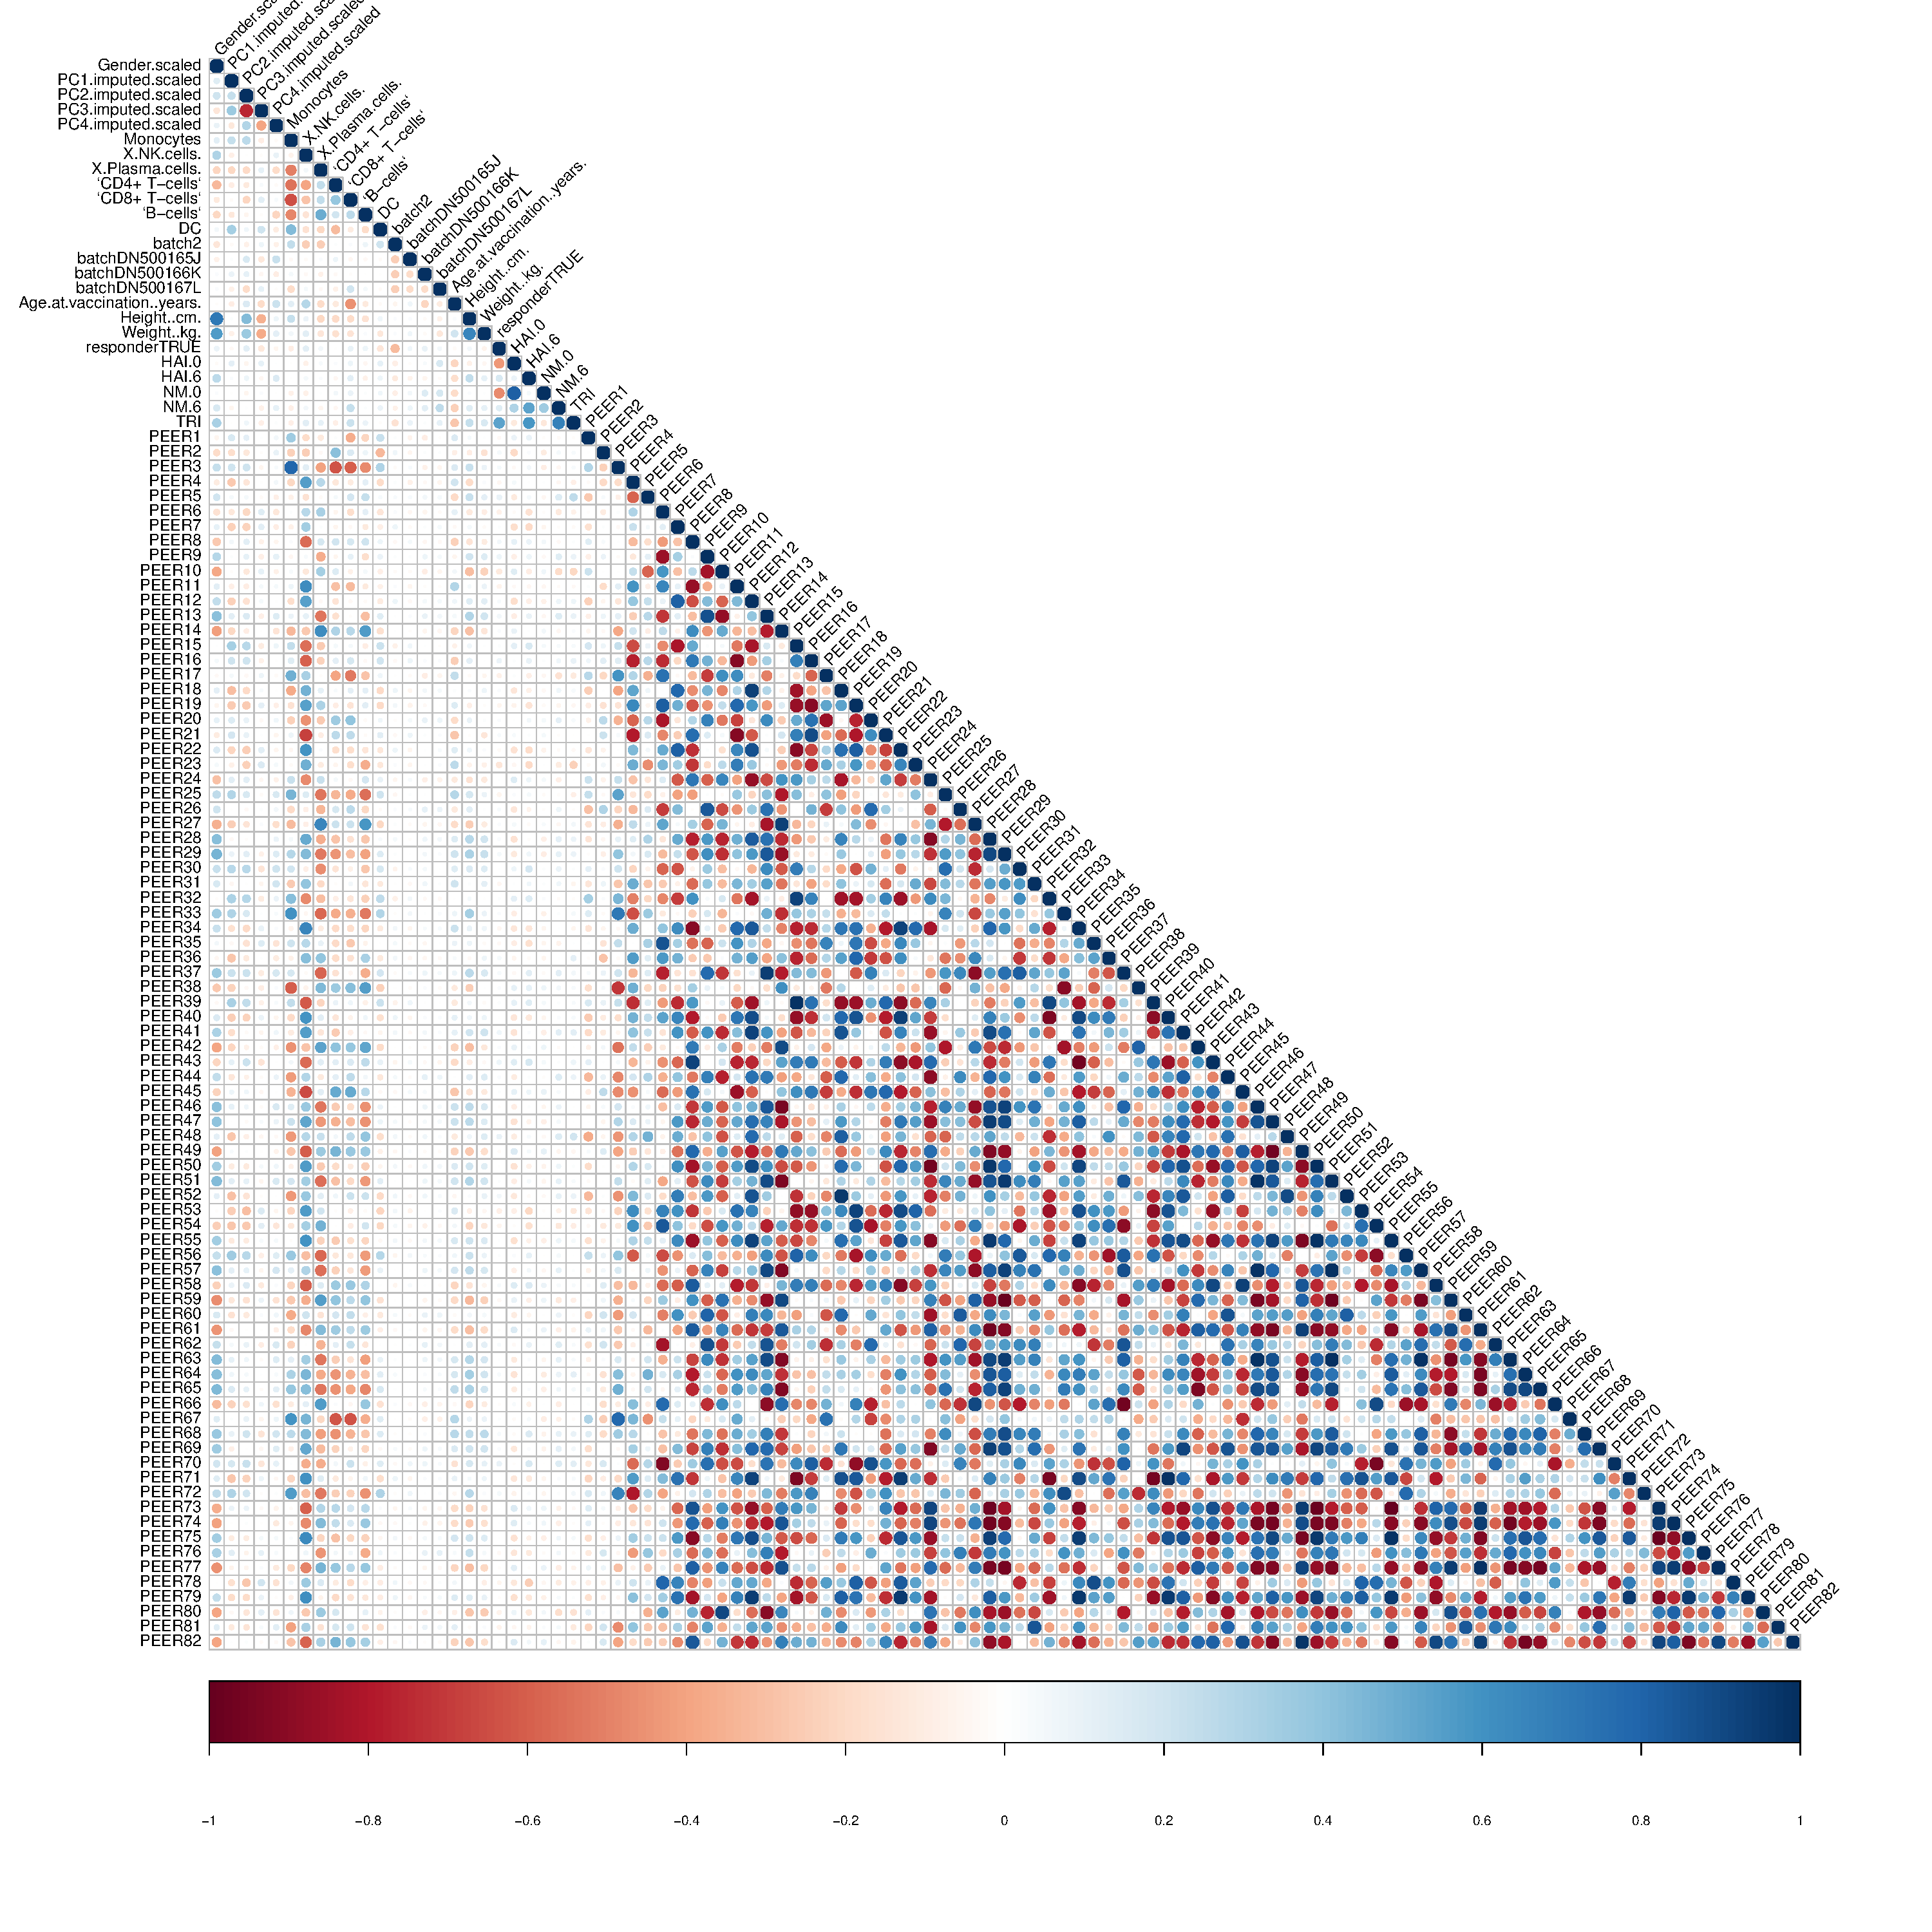
\includegraphics[width=1.0\textwidth,page=1]{mainmatter/figures/chapter_03/peer_mega/peer.factor_cor_matrix.v2.pdf}
    \caption{Correlation of PEER factors to known factors and other possible covariates. Note that PEER factors are not constrained to be orthogonal, so correlations to known factors are expected.}
    \label{fig:hird_peer_corMatrix_v2_mega}
\end{figure}
\todo{remake this with only top k factors, and prune the possible covariates}

\subsection{\glsfmtshort{eQTL} mapping per timepoint}

% 2.5.	Preprocess genotypes for limix
% 2.5.1.	Convert MAF filtered VCF -> 012 -> hdf5 format
% 2.5.1.1.	Do this for both strict 012 and continuous dosages
% 2.5.2.	Also convert 012 -> matrix eqtl SNP matrix format
% 2.5.2.1.	For eigenMT
% 2.5.3.	Parse out snpinfo and snplocs from VCFs
% 2.5.3.1.	Snpinfo for snp ids, for limix
% 2.5.3.2.	Snplocs for snp positions, and eigenMT
% 2.6.	Map eQTLs using limix 2.0, per timepoint
% 2.6.1.	Map cis-eQTLs within +- 1Mb of the gene start
% 2.6.1.1.	Phenotypes: per timepoint normalised input.expr from PEER script
% 2.6.1.2.	Covariates: sex, batch, 4 genotype PCs, 4 PEER factors
% 2.6.1.3.	Genotypes: MAF > 0.10 (in whole 169 individuals)
% 2.6.1.4.	Kinship: from LDAK, leave-one-chrom-out
% 2.6.2.	Output results in matrix eqtl-like output format
%
% For list of various methods considered, also see 2018-03-05, 2018-07-25, 2018-07-27 etc. in log
The performance of various software implementations of \glspl{LMM} specialised for genetic association studies are highly comparable; 
the specific choice of implementation can usually be made on the basis of computational efficiency\autocite{eu-ahsunthornwattana2014ComparisonMethodsAccount}.
I map \glspl{eQTL} within each timepoint using \software{LIMIX}\autocite{lippert2014LIMIXGeneticAnalysis}, which implements univariate and multivariate \glspl{LMM} with one or more random effects.

Imputed genotype probabilities were converted to continuous alternate allele dosages using bcftools (1.7-1-ge07034a).
Variants with sample $\text{\gls{AC}} < 15$ within each timepoint were excluded.
% TODO:
% per timepoint weakness here is that filtering MAF when unequal sizes restricts assessible results to lowest n
% but, due to tagging, not all hope is lost
\todo{add approximate MAFs, then cite hierarch paper}
% As is standard for imputation, we excluded all X-linked SNPs for the
% following reasons: (i) the X chromosome has to be treated differently from
% the autosomes; (ii) it cannot be predicted which allele is active on the X
% chromosome, (iii) testing males separately from females results in different
% sample sizes and power. Imputation of SNPs in the HapMap CEU population was
% performed using either MACH46 or IMPUTE47. All SNPs with a MAF <0.01 were
% excluded from analysis. In total, up to 2.11 million genotyped or imputed
% SNPs were analyzed.
% For example, an allele count of 1 in a female indi-cates a heterozygote
% genotype (one reference and onealternative allele), while a count of 1 in a
% male means only alternative allele exists and may cause more pro-found
% effects. The variance of the genetic effect may also differ between genders.
%
% X chromosome variants were excluded, as the number of copies differ between males and females, and X-inactivation makes it difficult to determine the active allele \url{https://www.nature.com/articles/ng.467},
% so sex-specific methods are required \url{http://www.biomedcentral.com/1471-2105/15/392}.
\todo{add note on treating x chrom variants with caution}

At each of 13570 genes, at all cis-variants within within $\pm \num{1}{Mb}$ of the gene \gls{TSS}, I fit the following model to map \gls{eQTL}:
% TODO
% Ensembl GENESEQSTART if fwd strand, otherwise GENESEQEND
 % Like all Ensembl features the start of an exon is always less than or equal to the end of the exon, regardless of the strand it is on. The start of the transcript is the start of the first exon of a transcript on the forward strand or the end of the last exon of a transcript on the reverse strand. The start and end of a gene are defined to be the lowest start value of its transcripts and the highest end value respectively.
\begin{equation}
\begin{split}
Y = 1 + sex + \sum_{i=1}^{4}{PC_i} + \sum_{}^{3}{xCell} + \sum_{i=1}^{k}{PC_i} + \beta G + \mathbf{u} + \epsilon
\end{split}
\label{eq:hird_reQTL_limix_model}
\end{equation}
\todo{lift proper vector notation from limix, then redo this with a timepoint subscript}
% TODO: kinship constrained varcov matrix. The scaling term is a var comp? error term has identity var cov
where the \gls{eQTL} effect size of interest is the slope of the genotype fixed effect $\beta$, the average additive effect of the alternate allele \autocite{visscher2019Fisher1918Paper};
and $\mathbf{u}$ is a random effect with zero mean and covariance matrix proportional to the \gls{LOCO} kinship matrix\footnote{For chromosome X variants, no \gls{LOCO} matrix is available from LDAK, so the matrix for chromosome 1 is used.}.
% The LMM requires a kinship matrix to scale the covariance matrix of the random effect mean zero and an unknown variance.
% In the past, the only available measure of genetic similarity was a kinship coefficient computed as a probability of identity by descent in a pedigree, and so a single random effect term sufficed to model genome-wide additive effects. Nowadays genetic similarity can be measured directly, and in many different ways, from genome-wide SNP data.
% GRM is : "consists of average allelic correlations across the SNPs (adjusted for LD and genotype certainty)" https://www.nature.com/articles/ng.3865?proof=true
% By default, LDAK scales kinships to have mean zero and average diagonalone
\todo{add formulation of the 0-mean random effect to show exactly how the kinship matrix is used \autocite{sul2018PopulationStructureGenetic}}
\todo{note stacking of kinship for day -7 repeated measures}

PEER factors are automatically weighted such that the variance of factors tends to zero as more factors are estimated, 
hence continuing to add more and more factors as covariates will not continue to improve \gls{eQTL} detection power, and eventually the model degrees of freedom will be depleted.
To optimise k, the number of factors to include as covariates%
\footnote{I avoid the commonly-performed two-stage approach of treating PEER residuals as expression phenotypes, as the degrees of freedom seen downstream will be incorrect, which can have a substantial effect on estimates at this modest sample size.}, 
% Also see \autocite{demissie2011BiasDueTwostage} % holmes2019ProblemsInterpretingUsing
Per-timepoint \gls{eQTL} mapping was performed in chromosome 1, iteratively increasing the number of factors until the number of \glspl{eQTL} detected plateaus.
I settled on a final choice of $k=10$ factors for pre-vaccination, 5 factors for day 1, and 5 factors for day 7 (\autoref{fig:hird_neGenesvsPeerK}).
\todo{i leave the pcs in to guard against unusually differentiated between pop markers, where random effect alone may not be enough \autocite{price2010NewApproachesPopulation}, \url{https://www.nature.com/articles/srep06874}}

\begin{figure}
    \centering
    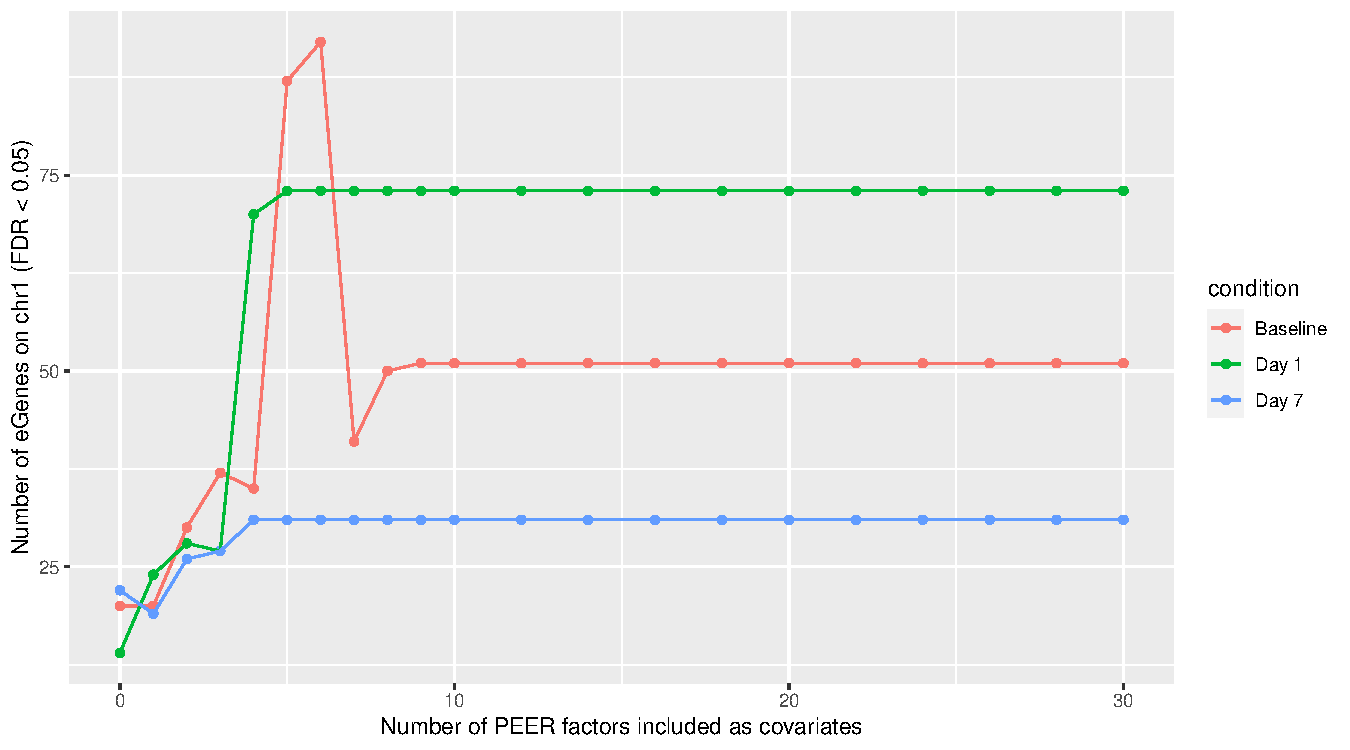
\includegraphics[width=1.0\textwidth,page=1]{mainmatter/figures/chapter_03/count_eGenes.signif_eGenes_vs_PEER_n.dataset_mega.chr_chr1.pdf}
    \caption{Number of significant eGenes detected on chromosome 1 (hierarchical Bonferroni-\gls{BH}\autocite{huang2018PowerFalseDiscovery} FDR < 0.05) as a function of the number of PEER factors included as covariates k.}
    \label{fig:hird_neGenesvsPeerK}
\end{figure}

\subsection{Joint \glsfmtshort{eQTL} analysis across timepoints}

% 2.10.	mashr
% 2.10.1.	Apply mashr to per-day meta-analysis beta/beta_ste results
Joint analysis was conducted with \software{mashr}\autocite{urbut2018FlexibleStatisticalMethods}, at 40197618 gene-variant pairs (mean of \num[round-mode=places,round-precision=0]{2962.24156227} tests per gene) for which summary statistics from within timepoint mapping were available in all three timepoint conditions.
\todo{recheck if did I do a SNPs only filter}
The mashr model incorporates multiple canonical (the identity matrix etc.) and data-driven covariance matrices to represent patterns of effects across conditions (in this case, $3 x 3$ matrices).
Data-driven covariance matrices are derived by dimension reduction of a strong subset of tests likely to have an effect in at least one condition.
I took the most significant variant per gene per condition, 
which ensures strong condition-specific effects are included (\autoref{fig:hird_mashr_strongSubset_Z_mega}), 
then further filtered to only nominally significant tests, resulting in a strong subset of 45962 tests.

\begin{figure}
    \centering
    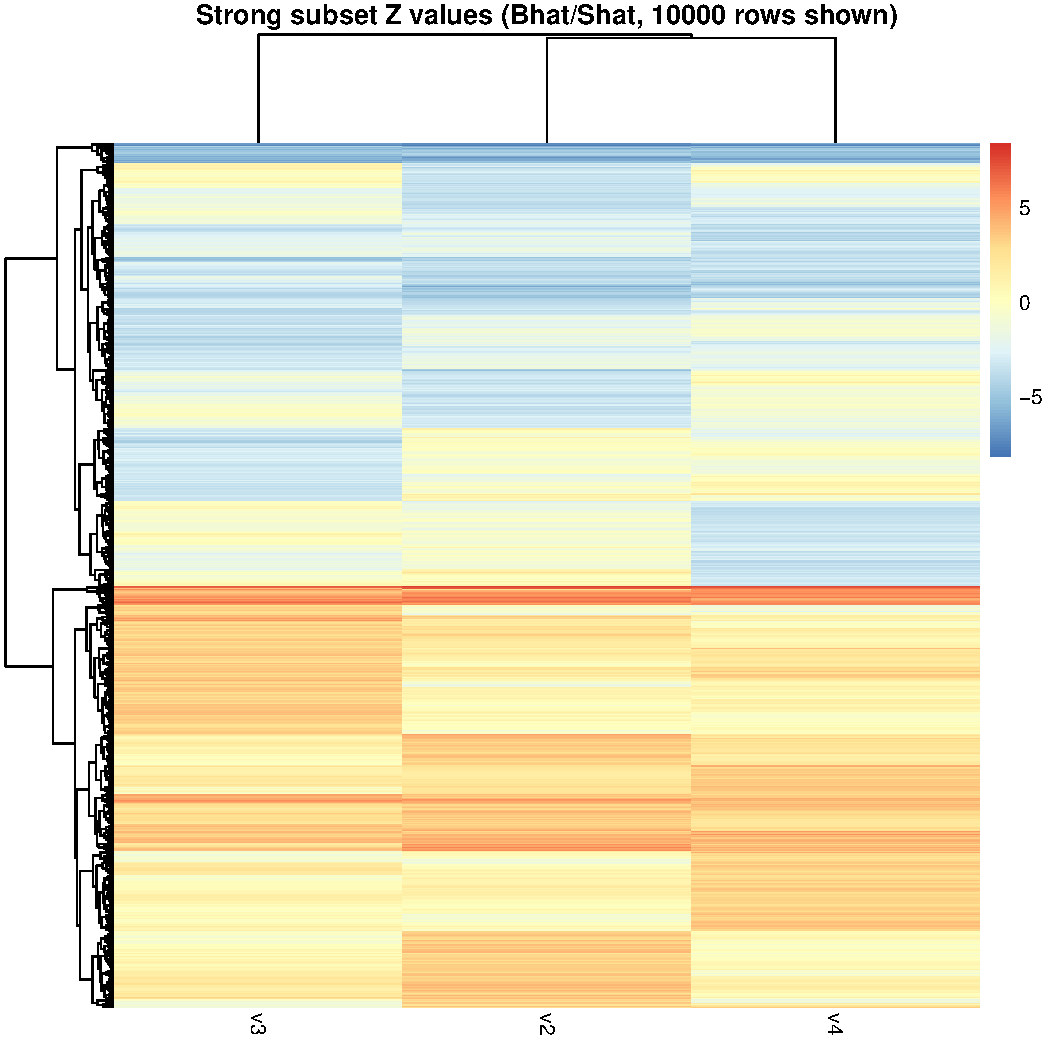
\includegraphics[width=1.0\textwidth,page=1]{mainmatter/figures/chapter_03/mash_mega/mashr.strong_subset_zval_heatmap.cisDist_1e6.sampleAcThresh_15.randomSubsetN_200000.pdf}
    \caption{Clustering of within-timepoint Z scores in the strong mashr subset (random sample of 10000/45962 tests), confirming the presence of strong condition-specific effects.}
    \label{fig:hird_mashr_strongSubset_Z_mega}
\end{figure}

The mash model was trained on a random subset of 200000 tests, using the Exchangeable Z-scores model\autocite{urbut2018FlexibleStatisticalMethods}.
The correlation of null tests between conditions, critical to account for due to the repeated measures structure of the data, was estimated using \software{mashr::estimate\_null\_correlation}.
\todo{note this is critical, since we know a priori not independent due to eqtl sharing}
The fitted model was used as a prior to compute posterior effects and standard errors for all tests through shrinkage.
% Stephens, M. (2016). False discovery rates: A new deal. Biostatistics, kxw041. https://doi.org/10.1093/biostatistics/kxw041
% analogous to a false discovery rate, but more stringent because it requires true discoveries to be not only nonzero, but also correctly signed.
%
% Also see:
% type s error rates for classical and bayesian single and multiple comparison procedures
% Why We (Usually) Don’t Have to Worry About Multiple Comparisons (2012)
% Beyond Power Calculations: Assessing Type S (Sign) and Type M (Magnitude) Errors (2014)
A condition-specific Bayesian measure of significance \gls{lfsr} is returned, which can be interpreted as the the probability given the data, that the declared sign of the effect is incorrect.
\todo{move lfsr explanation prior to ashr in dge chapter}

\subsection{Defining shared and response eQTLs}

Many of the tested variants for each gene will be in high \gls{LD}.
% qtls.merged[, signif_rank := frank(qtls.merged, lfsr, -INFO, -MAF_sample, SNP_gene_TSS_dist, POS)]
To unambiguously select a lead \gls{eQTL} variant per gene, I selected the variant with the lowest lfsr in any condition, 
breaking ties by highest imputation INFO, highest \gls{MAF}, most upstream of the \gls{TSS}, and genomic coordinate.
Sharing was then evaluated for that gene-variant pair across all three conditions.

Thresholding on the lfsr is not appropriate for determining sharing, as the difference between significant and non-significant effect estimates in two conditions is not necessarily significant\autocite{schenker2001JudgingSignificanceDifferences,gelman2006DifferenceSignificantNot}.
% Not just use lfsr thresholds:
\autocite{urbut2018FlexibleStatisticalMethods} provides a heuristic that two effects are shared by magnitude if they have the same sign, and are also within a factor of 2 of one another,
but this does not consider the posterior standard error of the estimates.
% Also see:
% https://andrewpwheeler.wordpress.com/2016/10/19/testing-the-equality-of-two-regression-coefficients/
    % Var(A-B) = Var(A) + Var(B) - 2*Cov(A,B)
    % NOTE: Assumes that Cov is 0, this is anticonservative when Cov is actually positive.
% Also: notes from 2018-10-11 on wald test, and comments on sharing_func in get sharing script
% Also: USING THE CORRECT STATISTICAL TEST FOR THE EQUALITY OF REGRESSION COEFFICIENTS https://onlinelibrary.wiley.com/doi/abs/10.1111/j.1745-9125.1998.tb01268.x
Between a pair of effects in two conditions, I compute a z-score for the difference in effects\autocite{clogg1995StatisticalMethodsComparing,schenker2001JudgingSignificanceDifferences}:

\begin{equation}
z = \frac{\beta_x - \beta_y}{\sqrt{\sigma_x^2 + \sigma_y^2 - 2\sigma^2(x, y)}}
\end{equation}

This strategy has been applied to call reQTLs by \autocite{kim-hellmuth2017GeneticRegulatoryEffects},
% Actually we can get:
% PosteriorCov
% Q x Q x J array of posterior covariance matrices, if the output_posterior_cov = TRUE.
assuming posterior pairwise covariance of effects is zero $\sigma^2(x, y)$.
\todo{not sure whether this is conservative or anti-conservative}
\todo{mashr does not provide by default}
% TODO we consider the var cov matrix of coefficients here, not the expressions
% TODO this is convservative unless corr is >0.5?
% NOTE: A Wald test uses W ~ chisq(1), equivalent to sqrt(W) ~ N(0, 1).
A Wald test \pvalue{} for the difference can be computed, as under the null hypothesis of zero difference, asymptotically $z \sim \mathcal{N}(0, 1)$.
I use nominal \pvalue{} < 0.05 as a heuristic threshold (like the mashr recommended 2-fold threshold) to define reQTL effects that are strong, rather than a formal measure of significance.
% TODO: but ideally, define reQTL strength as an ordering, not by thresholding
% TODO: emph the progression from simple lfsr (e.g. gtex ccqtl, huang2020NeonatalGeneticsGene) -> mashr 2-fold (mashr) -> to want to look at se too
Effects are only compared if at least one of the two effects has lfsr < 0.05, to avoid sharing being driven by null effects.

\subsection{Replication of eQTLs in a reference dataset}

To validate the \gls{eQTL} mapping approach, I estimate the replication of significant eQTLs in a large independent reference.
Due to the lack of large sample size \gls{eQTL} maps specific to \gls{PBMC}, I use the GTEx v8 whole blood dataset as my reference dataset (n=670, 51.2\% eGene rate).
For lead variants called as significant in the \gls{HIRD} dataset at a given lfsr threshold, I lookup the nominal \pvalue{} for that variant in GTEx (where the variant exists in both datasets).
I applied \software{qvalue::qvalue\_truncp} to estimate the proportion of those GTEx nominal \pvalues{} that are null ($\pi_0$), the compute a measure of replication $\pi_1 = 1 - \pi_0$.

The mega-analysis has comparable replication rate to \gls{RNAseq}-only analysis for shared \glspl{eQTL} at moderately stringent \gls{lfsr} thresholds up to $10^{-5}$ (\autoref{fig:hird_eQTL_pi1vsGTExWholeBlood}).
Past this, as the $\pi_1$ procedure assumes a well-behaved \pvalue distribution in $\left[0, 1\right]$, 
reliability declines due to the number of \pvalues{} being too small\footnote{\url{https://github.com/StoreyLab/qvalue/pull/6\#commitcomment-26277751}}, or the maximum \pvalue{} being too far from 1.
The numbers of \glspl{reQTL} were too low to assess replication using this method, and one might not expect them to replicate in a baseline dataset such as GTEx whole blood, especially for those \glspl{reQTL} significant only at post-vaccination timepoints.
As the mega-analysis has a higher eGene rate (\percentage{0.5075166} vs. \percentage{0.29914529915}) compared to the \gls{RNAseq}-only analysis, with similar replication,
I assume this represents a power advantage from having larger a sample size, rather than technical effects from merging the expression data.
% \todo{add comment on number of eGenes. the real reason here is prob robustness?}
\todo{RNAseq does test about 7000 more genes though...}
% TODO: this approach may overestimate the replication rate as it does not take the direction or magnitude of eQTL effects into account.

\begin{figure}
    \centering
    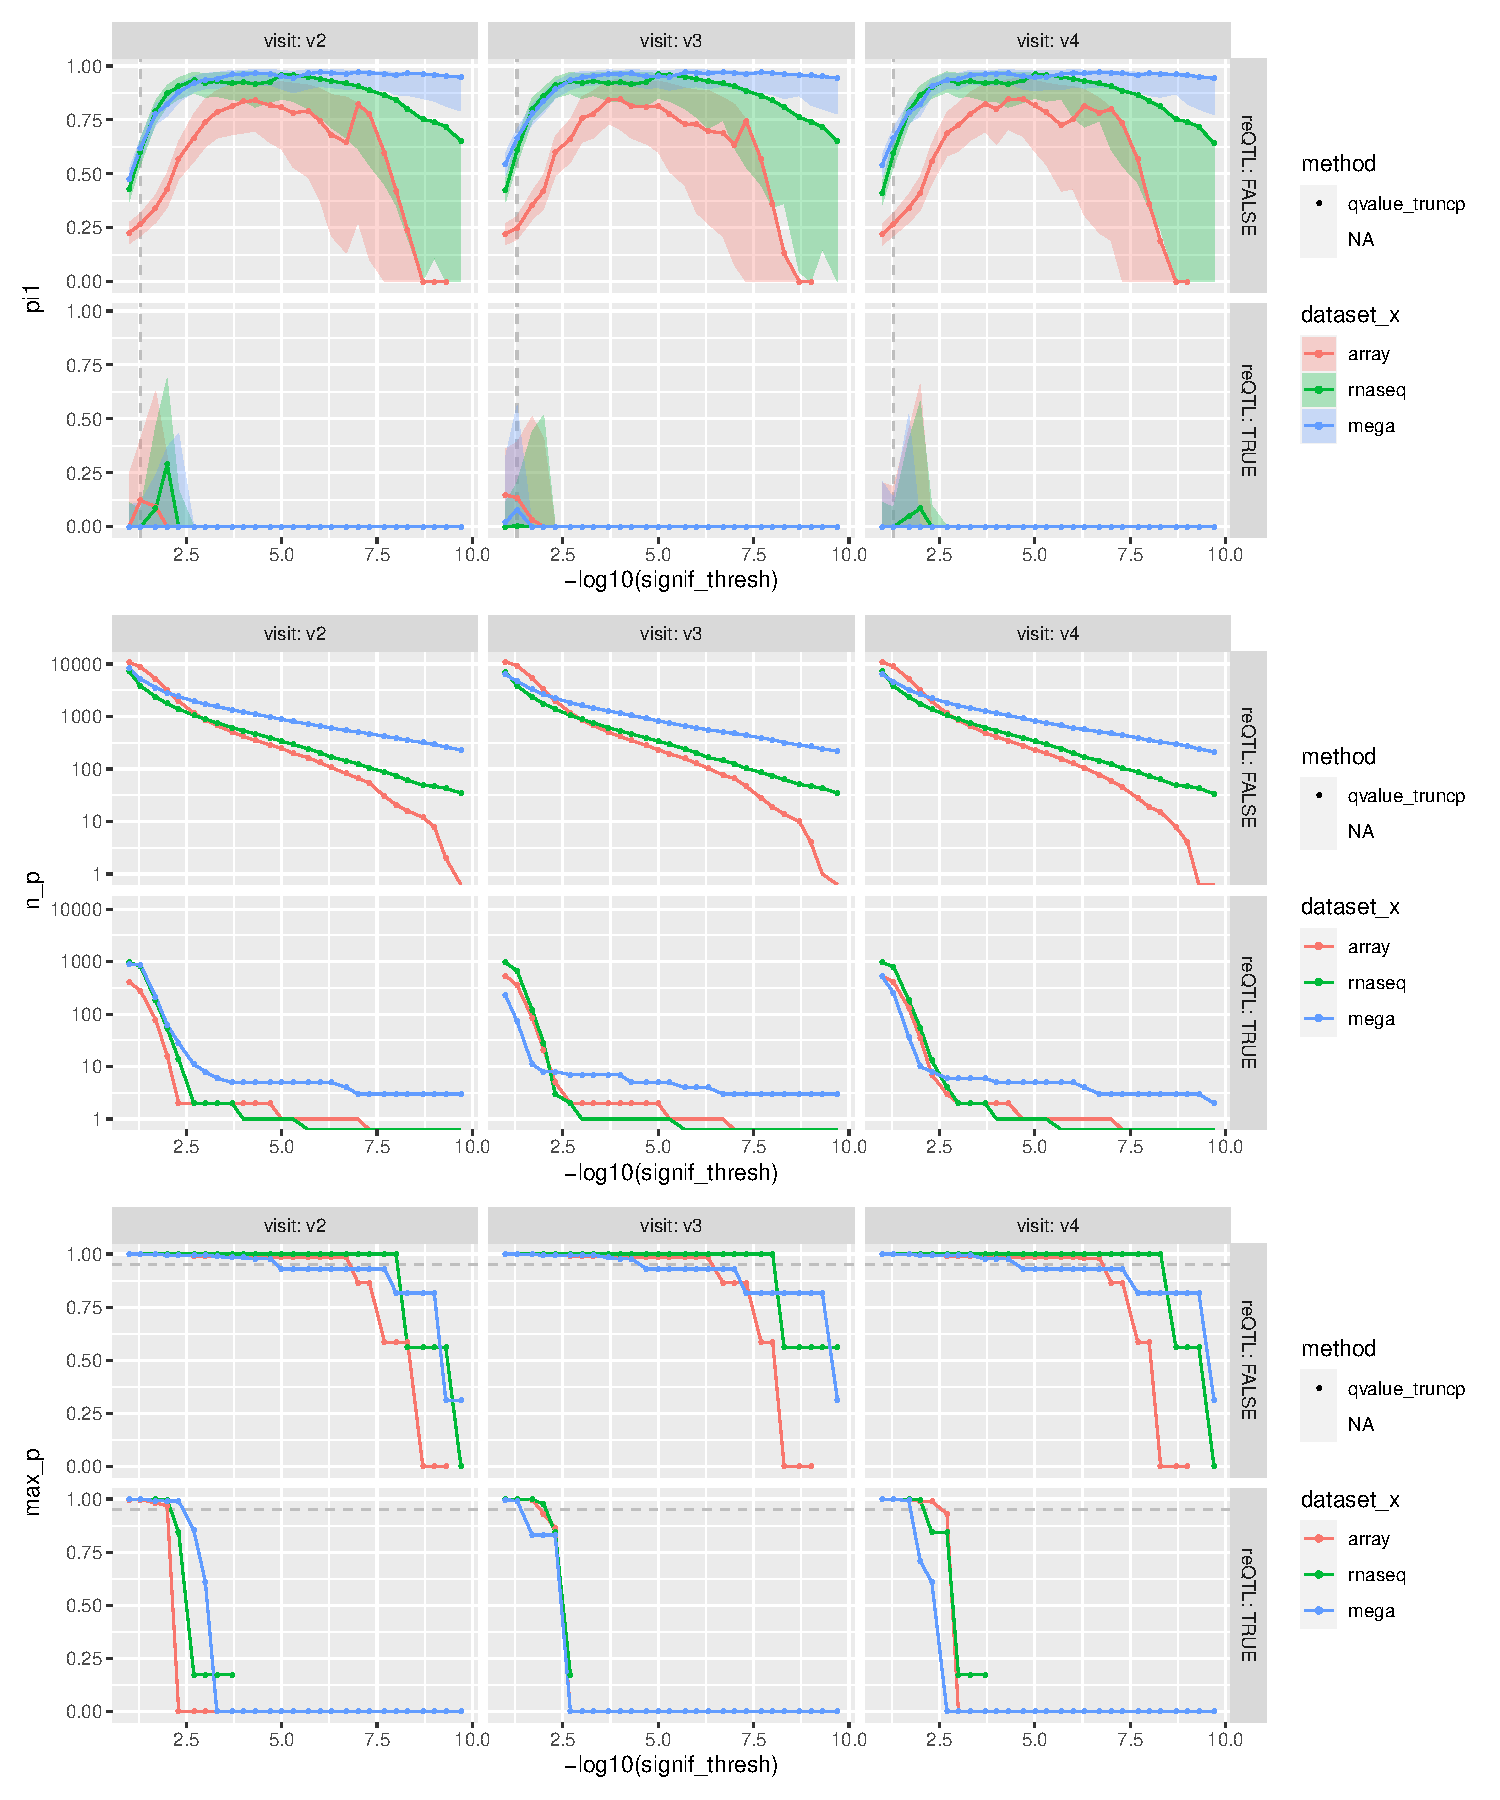
\includegraphics[width=1.0\textwidth,page=1]{mainmatter/figures/chapter_03/compute_pi1.pi1_by_thresholds.pdf}
    \caption{
        Effect of \gls{HIRD} lfsr threshold on GTEx whole blood replication rate ($\pi_1$), number of \pvalues{} used to compute $\pi_1$, and maximum \pvalue{} among those \pvalues{}; 
        for shared and \gls{reQTL} called from the array-only, \gls{RNAseq}-only and mega-analysis pipelines. 
        Shaded region for $\pi_1$ represents the 5th-95th percentile range of 1000 bootstraps.
    }
    \label{fig:hird_eQTL_pi1vsGTExWholeBlood}
\end{figure}
        % TODO: 10000?

\subsection{Genotype interactions with cell type abundance}
\label{subsec:hird_reQTL_methods_cellTypeInteraction}

% TODO: note moderator is more likely, but mediator G -> CC -> E is also possible

% TODO need a DAG on why reqTL in vivo cannot guarantee causality of G on change in E

\todo{be more specific: "moderator", 'modify'?????}
% TODO: In regression, one of the assumptions is the additive assumption. This assumption states that the influence of a predictor variable on the dependent variable is independent of any other influence
% Holding all else equal Implies beta does not depend on other predictors
% https://journals.lww.com/epidem/Fulltext/2009/11000/On_the_Distinction_Between_Interaction_and_Effect.16.aspx
% https://significantlystatistical.wordpress.com/2014/12/12/confounders-mediators-moderators-and-covariates/
% TODO: why?
% happens if there is cell type specific relevance of g
% cause cell type affects g->e i.e. symetrically, geno affects c -> e
% Figure out what DAG model causes a reQTL in bulk to not represent causality of G -> change in e
If the abundance of a particular cell type does truly modify the \gls{eQTL} effect, 
then an interaction term between genotype and cell type abundance is required,
\todo{point is, doesn't make sense to assume the genotype effect is the same at all levels of cell type abundance}
% TODO: what is the effect of genotype going up a unit holding cell props constant? well, actually it depends on the constant....
% i.e. this is non-addititivty 
otherwise the regression slope of the \gls{eQTL} term will be biased;
% TODO: OVB by setting interaction coefficient to zero
% http://consirt.osu.edu/wp-content/uploads/2014/10/CONSIRT-Working-Papers-Series-9-Mikucka_Sarracino_Dubrow.pdf
% Most importantly, the figures document thatwrongly  omitting  an  interaction  term  (Figure  3)  can  bias  the  estimates  much  more  thanwrongly including an interaction term (Figure 4).
one can not adjust for this modification just by including the main effect for cell type abundance.
% TODO: if the data gen process is so, the simply a misspecification to not have it
% referred to in econometrics as "functional form misspecification", a special case of OVB.
% e.g. https://www.econometrics-with-r.org/9-2-ttivomra.html
% basically, if you need a diff slope over levels of modifying var, it can't possibly have one without it being in the model
% if you need var slopes, but only allow var intercepts
%
% https://stats.stackexchange.com/questions/263324/how-can-the-regression-error-term-ever-be-correlated-with-the-explanatory-variab
% the realisation of the error term, the residuals, is forced to be uncorrelated, hence you get a biased estimate
Given the modest sample size, I use the two-step approach used by others\autocite{westra2015CellSpecificEQTL,peters2016InsightGenotypePhenotypeAssociations,kim-hellmuth2017GeneticRegulatoryEffects,davenport2018DiscoveringVivoCytokineeQTL},
where tests for interaction are only performed at a subset of tests, often the lead \gls{eQTL} variant for each gene.
% Unfortunately, there seems to be no consensus between these studies for controlling the interaction effect tests for multiple testing.
%
% Strange custom 5% FDR: westra2015CellSpecificEQTL
% Bonferroni: kim-hellmuth2017GeneticRegulatoryEffects
% Benjamini-Hochberg FDR: kim-hellmuth2017GeneticRegulatoryEffects
% Benjamini-Hochberg procedure, and a 0.15 FDR threshold: peters2016InsightGenotypePhenotypeAssociations
%
% https://www.jmp.com/support/help/en/15.2/index.shtml#page/jmp/effect-heredity.shtml
% The principle of effect heredity relates to the inclusion in the model of lower-order components of higher-order effects. The motivation for this principle is observational evidence that factors with small main effects tend not to have significant interaction effects.
% NOTE: this is not strictly effect heredity, as I do not consider the significance of cell proportion terms
%
% TODO: dodgy, review this paper again
The key to the two-stage approach is that if the estimates for the interaction effect are sufficiently independent from the estimates of the main effect from main-effect only models,
the type I error can be controlled based on the number of interactions that are actually tested, rather the number of interactions that could have been tested for\autocite{kooperberg2008IncreasingPowerIdentifying,peters2016InsightGenotypePhenotypeAssociations}.
It is unclear whether this assumption holds, as the size of the main effect may contribute to power for detecting interaction effects.
As the main purpose of the interaction analyses is scanning for cell type effects at detected \glspl{reQTL},
I chose to test for interactions only at the lead \gls{eQTL} variant for each gene with a significant main \gls{eQTL},
then apply the \gls{BH} \gls{FDR}, as used by others\autocite{peters2016InsightGenotypePhenotypeAssociations,kim-hellmuth2017GeneticRegulatoryEffects}.

Models in interactions between genotype and other predictors were fit using \software{lme4qtl}.
The model specification identical to \autoref{eq:hird_reQTL_limix_model}, with the addition of three interaction terms between genotype and each xCell score.
Significance is assessed using the likelihood-ratio test versus the nested model with no interaction terms.
\todo{can we interpret with peer in? add note of CLAIM here that although peer is correlated with xcell, interactions are only formed with xcell, so the interaction term can be interpreted per unit of genotype increase when xcell=0}

\subsection{TODO Statistical colocalisation}

% TODO
% Choice of method;
% See coloc_comparisons in notes for a summary
% Coloc and assumptions; Hypercoloc and assumptions
%
\todo{this analysis is incomplete, and is one of the things I would suggest to round off this chapter}
- if adding coloc analysis, add \url{https://github.com/jrs95/hyprcoloc} methods here
- cannot deal with multiple causal within each group

\section{Results}

\subsection{Mapping reQTLs to Pandemix vaccination}

Within each timepoint condition (day 0 pre-vaccination, day 1, and day 7), cis-\glspl{eQTL} ($\pm 1 \text{Mb}$ of the \gls{TSS}) were mapped using \software{LIMIX},
then joint analysis of effects was done using \software{mashr} to obtain posterior effect size and standard errors.
At \gls{lfsr} < 0.05, 6887/13570 genes (\percentage{0.5075166}) were eGenes (genes with a significant \gls{eQTL}) in at least one timepoint.
To sidestep the issue of multiple tested variants per gene being in \gls{LD},
the most significant \gls{eQTL} variant across all timepoints was selected as the lead variant for each eGene,
then \glspl{reQTL} were defined by comparing the effect size of this lead \gls{eQTL} between each pair of timepoints.
Most \glspl{eQTL} were shared across timepoints; 1154/6887 (\percentage{0.1675621}) \glspl{eQTL} were classified as \glspl{reQTL} between any pair of timepoints (nominal p difference < 0.05).
% 1131 if ignoring d1 vs d7
% \todo{might be interesting to note not so many d1 vs d7 reQTL}
% TODO: expected? in fairfax, how many shared? in vivo studies, more or less?
% look at ackermann2013ImpactNaturalGenetic for list of sharing estimates
\todo{if it would be interesting to compare the sharing estimate condition by condition approach to mashr, then redo and pull in eigenmt-bh values}

\autoref{fig:hird_eQTL_upset_mega} illustrates the difference between calling sharing using a significance threshold versus difference in betas approach.
For instance, day 0 was the timepoint with the largest number of eGenes, reflecting the larger sample size compared to other timepoints.
Although there are 1427 eGenes significant at only day 0, there are only 646/1427 reQTL among them, as the effect size at day 0 does not differ significantly when compared to day 1 or day 7 for the remainder.
The strongest \glspl{eQTL} with the highest \gls{PVE}\footnote{TODO: add to methods \url{https://journals.plos.org/plosone/article/file?type=supplementary&id=info:doi/10.1371/journal.pone.0120758.s001}}
are shared between timepoints, highlighting the power advantage for mapping shared effects granted by joint analysis.
% \todo{put pve formula in methods, include point that pve is (very rough) norm to var(y), so can compare between timepoints and genes with different MAF and raw variance}
\todo{actually, i've found that my PVE approximation is basically rescaled abs(Z), so pve is a bit pointless if we already have z, and doesn't really help with comparability between genes with diff var/MAF}

\begin{figure}
    \centering
    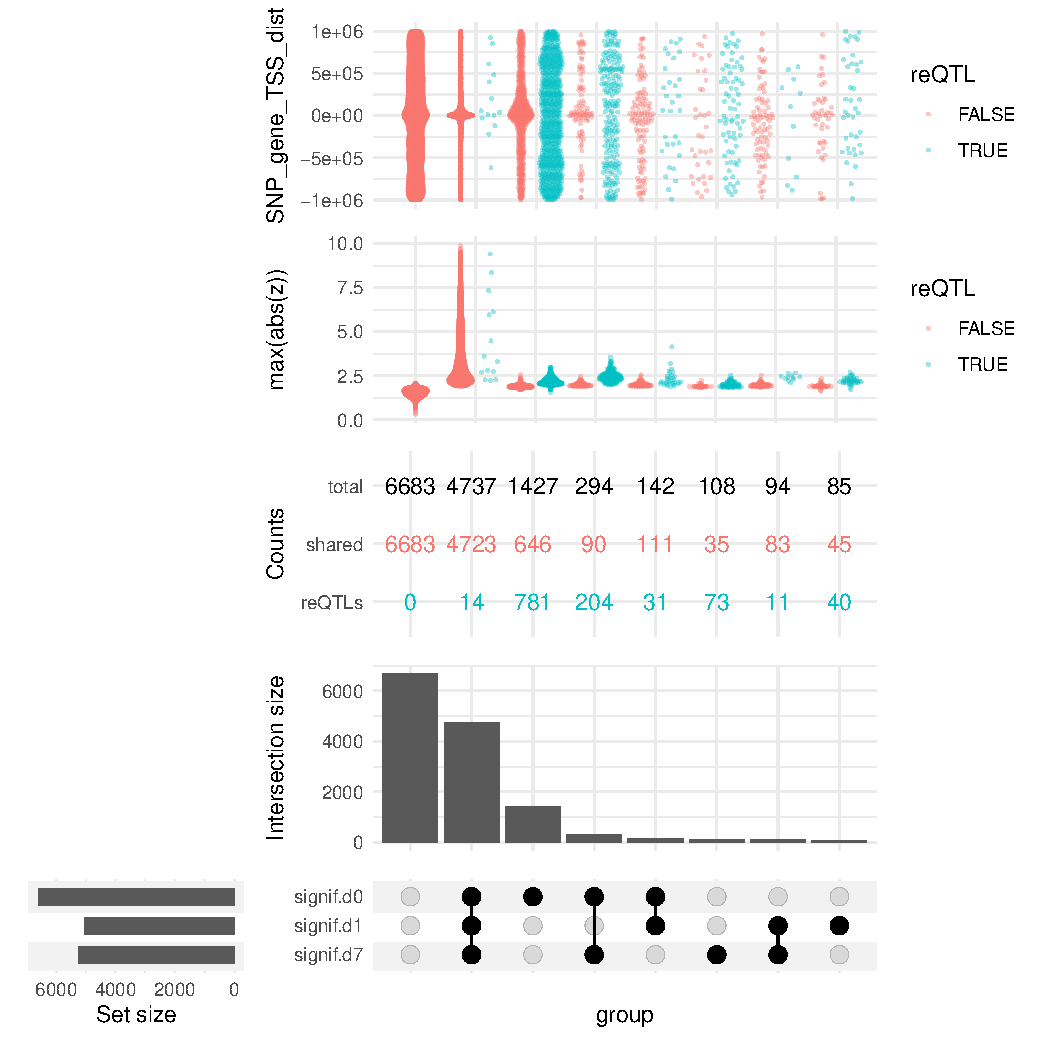
\includegraphics[width=1.0\textwidth]{mainmatter/figures/chapter_03/compare_dge_eqtl.upset.pdf}
    \caption{
        Summary of eQTL mapping results at 13570 genes-lead eQTL pairs,
        with intersections based on significance (lfsr < 0.05).
        Counts of shared eQTLs and reQTLs; and distribution of INFO score, min MAF across timepoints, and max PVE across timepoints for those lead variants are shown above each intersection.
    }
    \label{fig:hird_eQTL_upset_mega}
\end{figure}

\subsection{Characterising reQTLs post-vaccination}

As detection power is greatest at day 0, 
I focus on \glspl{eQTL} that are reQTLs between day 0 and either day 1 or day 7 post-vaccination, 
% NOTE: the apparent gap is filled by dampening effects that are n.s. in day 1/7
and are significant at the corresponding timepoint:
\todo{requiring signif post-vaccination may not be correct, as it excludes many dampening effects}
819 reQTL between day 1 and day 0, 
and 1002 reQTL between day 7 and day 0 (\autoref{fig:hird_eQTL_zSharing_vs_TSSdist_mega}).
Gene set enrichment analysis on the eGenes targets for these sets of \glspl{reQTL} did not detect any significant enrichments (\software{gprofiler2}, g:SCS adjusted p < 0.05).
%
% if so, then define mag,damp,flip
% Of the 819 reQTL between day 1 and day 0, there 49 magnifiers, 720 dampeners, 39 sign flips.
% Of the 1002 reQTL between day 7 and day 0, there are 58 magnifiers, 651 dampeners, 211 sign flips.
% \todo{could put in reqtl ranked cerno enrichments here}
% \todo{put cerno on pve/abs(z) e.g. hla ranked enrichments, then comment on strong shared effects in discussion}
%
Many of the \gls{reQTL} that satisfy this criteria have opposite effects pre- and post-vaccination---as lfsr quantifies uncertainty in the sign of the effect, I do not compare the sign unless the reQTL is also significant at day 0.
Shared \glspl{eQTL} are enriched close to the \gls{TSS}, whereas \glspl{reQTL} are distributed across the cis- window.
\todo{the lack of any positional enrichment makes me concerned for false positives? check with ASE?}
% TODO: another possiblility
% GARFIELD enrichment analysis21 showed that the cis-eSNPs were enriched in 3′ untranslated regions (UTR), 5′ UTR, and exon regions (Supplementary Fig. 4), consistent with known mechanisms of cis-eQTLs.

%
% Possible Ranking metrics for ranked enrichments
%     PVE: prefers large maf and high betas since it squares the beta. even if the beta does not change so much. ignores sign.
%     beta:
%     p: ignores sign
%     Z score:

% \todo{double check magnifier definition relative to DGE}
\begin{figure}
    \centering
    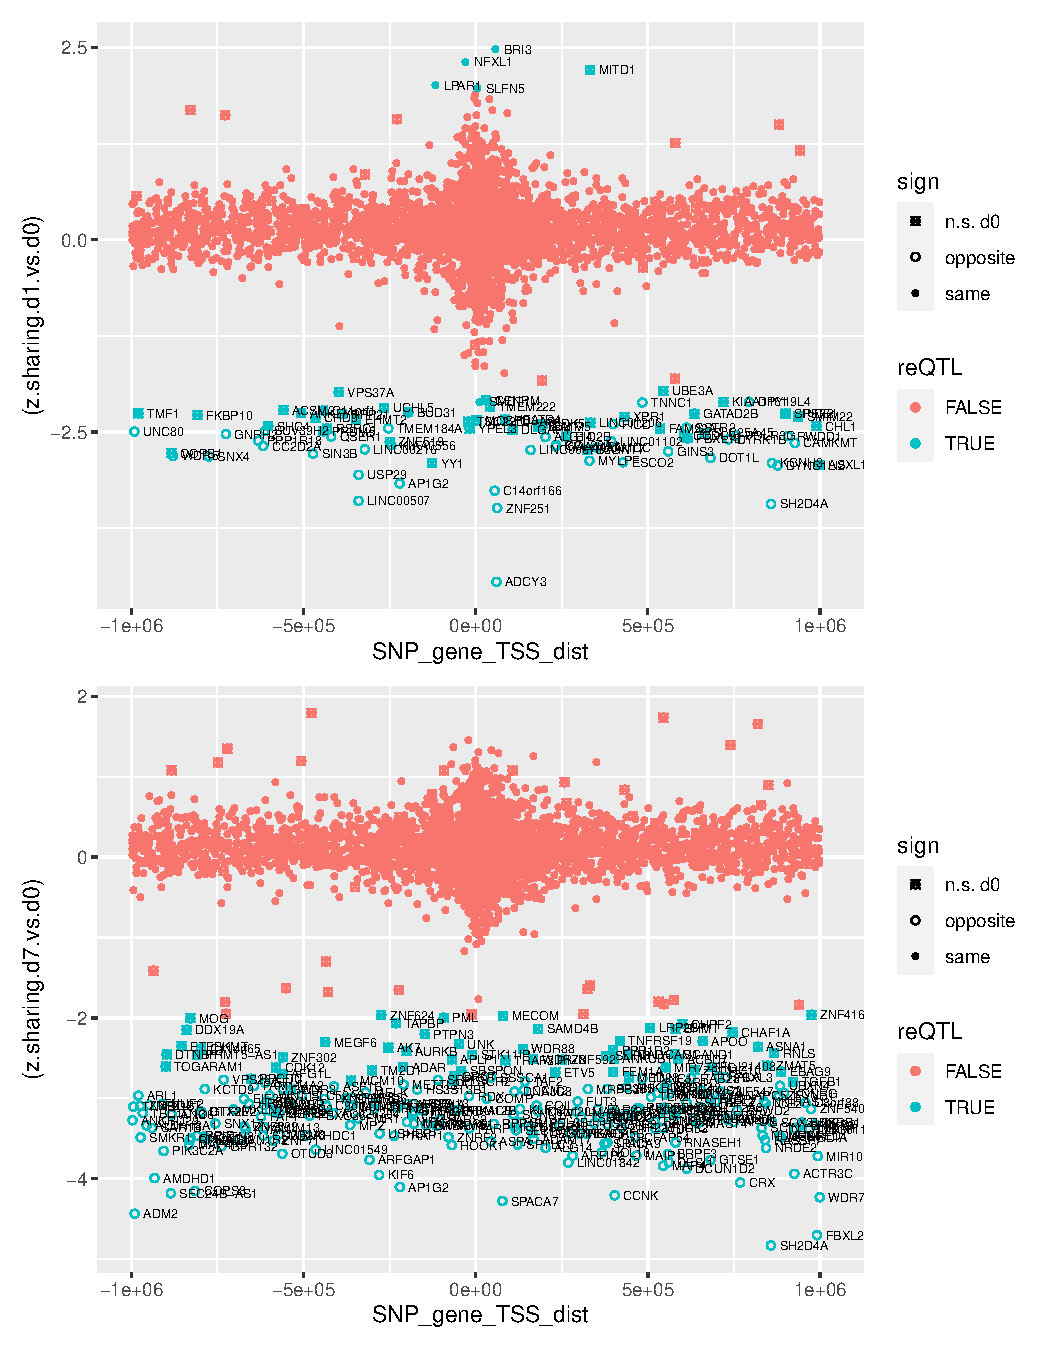
\includegraphics[width=1.0\textwidth]{mainmatter/figures/chapter_03/compare_dge_eqtl.z_sharing.vs.SNP_gene_TSS_dist.pdf}
    \caption{
        Z score for difference in effect vs. day 0, of lead eQTLs for all eGenes significant at either day 1 or day 7;
        versus distance of the lead SNP to the TSS.
        Direction of effect is aligned so that the beta at day 0 is positive. 
        Points with positive z score are magnified effects post-vaccination, points with negative z scores are dampening and opposite sign effects.
    }
    \label{fig:hird_eQTL_zSharing_vs_TSSdist_mega}
\end{figure}

\todo{expand this to plot 1, list top 5 damp, flip, amp at each timepoint}
\todo{note anything in lit about any of the 30}
The strongest reQTL at day 1 was for \gene{ADCY3} (p difference = \num{8.676917e-06}, BH FDR = \num{0.1177458}),
where the \gls{reQTL} variant explained approximately \percentage{0.01862996} of expression variation at day 0, increasing to \percentage{0.14075782} at day 1 (\autoref{fig:hird_eQTL_ploteQTL_ADCY3}).
At day 7 the strongest \gls{reQTL} was at \gene{SH2D4A} (p difference = \num{1.369564e-06}, BH FDR = \num{0.01747935}).
Here, the \gls{reQTL} variant explained similar amounts of expression variation at day 0 (\percentage{0.08229266}) and day 7 (\percentage{0.08956865}), with opposite directions of effect (\autoref{fig:hird_eQTL_ploteQTL_SH2D4A}).
Both \gene{ADCY3} and \gene{SH2D4A} have moderately high percentile expression at all timepoints, and are not differentially expressed post-vaccination.
Overall, compared to genes without reQTL,
% \todo{change % to reflect new numbers}
% TODO: dge by reqtl plot
% TODO: need to compare to shared eQTL
\glspl{reQTL} were less likely be differentially expressed post-vaccination at day 1 (\percentage{0.2649573} for reQTL vs. \percentage{0.4227119}, Fisher's test p < \num{2.2e-16}),
\todo{reword not significant}
and no significant difference was observed at day 7 (\percentage{0.02195609} for reQTL vs. \percentage{0.01368555}, Fisher's test p = \num{0.05088}).
% Overall, \glspl{reQTL} were less likely compared to shared \glspl{eQTL} (\percentage{0.2920277} vs. \percentage{0.4929356}, Fisher's test p < \num{2.2e-16}) to be differentially expressed post-vaccination.
Only 5/68 (\percentage{0.1323529}) genes with \glspl{reQTL} that explain more variation at day 1 were upregulated at day 1 vs. day 0; 5/226 (\percentage{0.02212389}) for day 7 vs. day 0.
\todo{double check denoms}

\begin{figure}
    \centering
    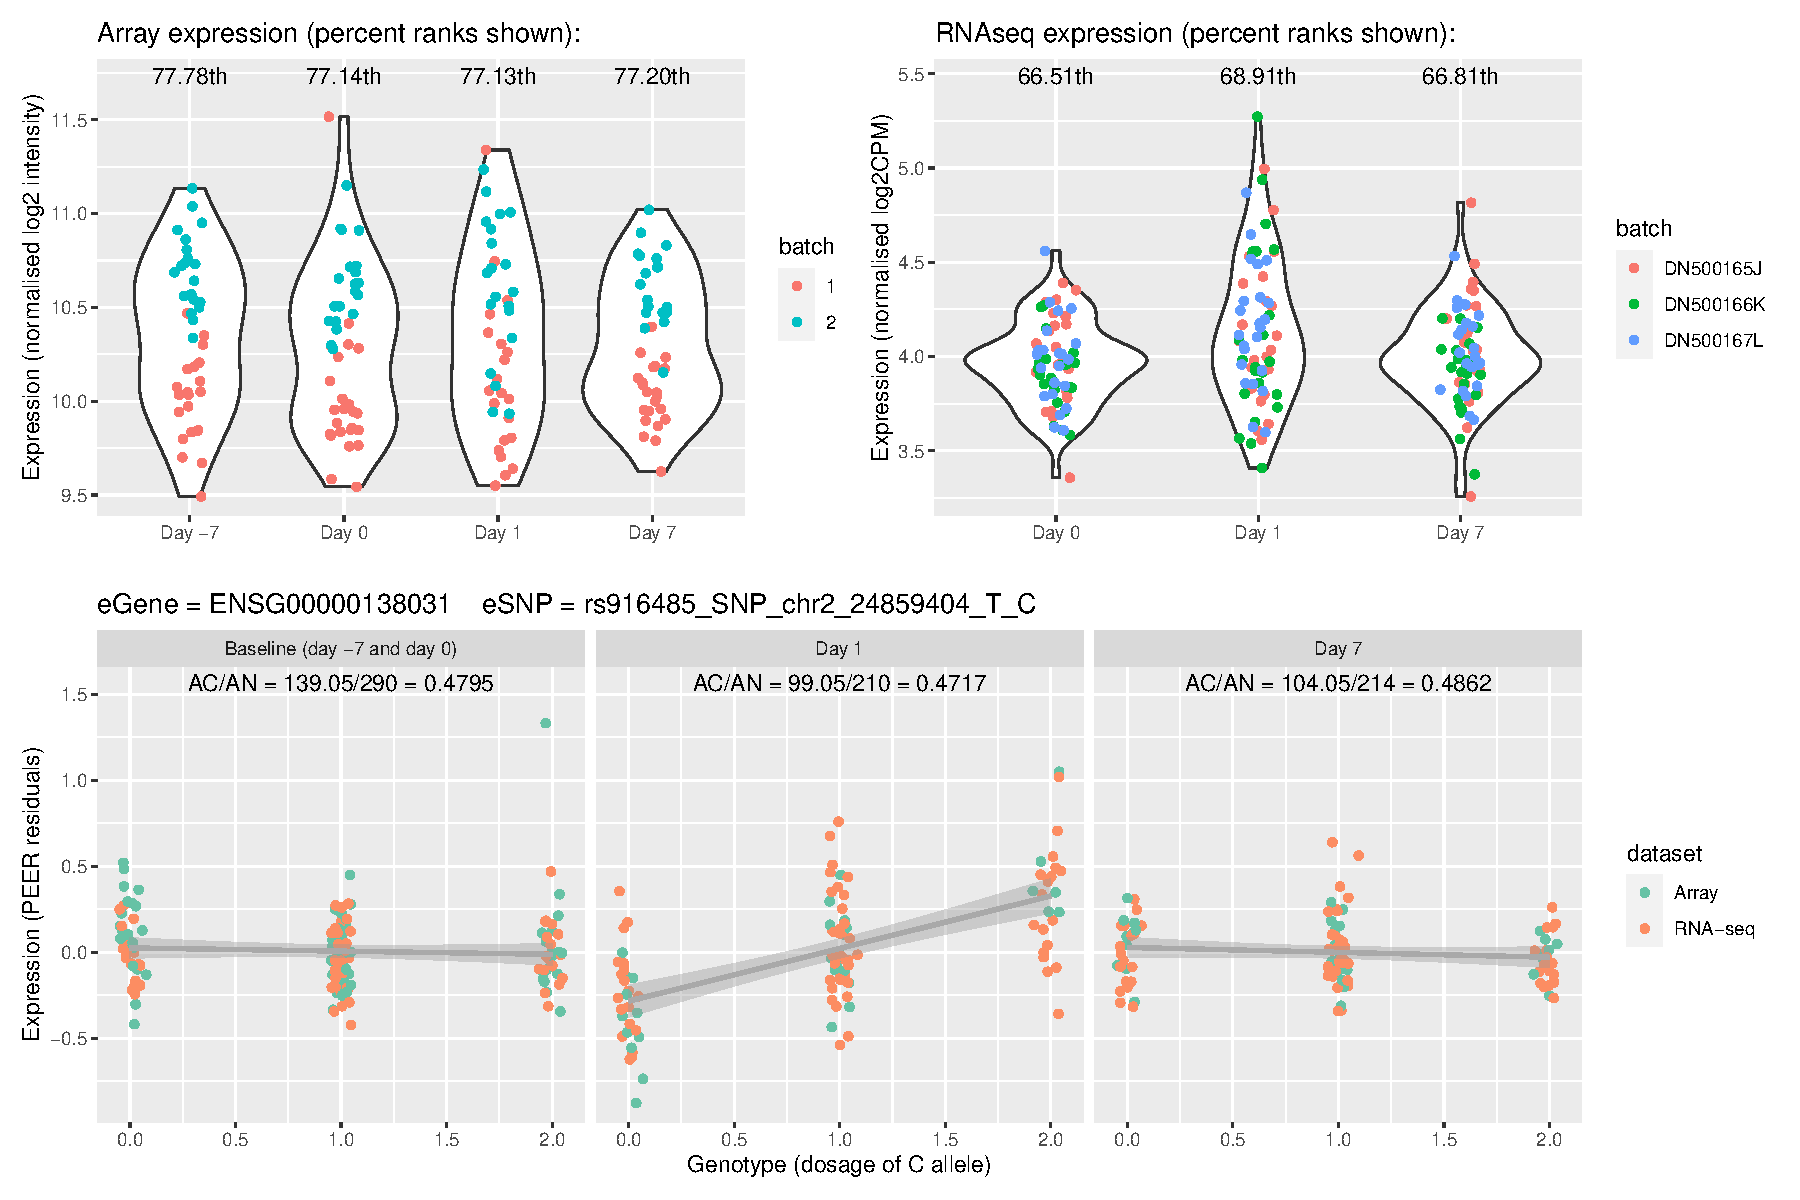
\includegraphics[width=1.0\textwidth,page=1]{mainmatter/figures/chapter_03/plot_dge_eqtl_genotypes.ENSG00000138031,rs916485_SNP_chr2_24859404_T_C.pdf}
    \caption{\gene{ADCY3}, strongest reQTL at day 1.}
    \label{fig:hird_eQTL_ploteQTL_ADCY3}
\end{figure}

\begin{figure}
    \centering
    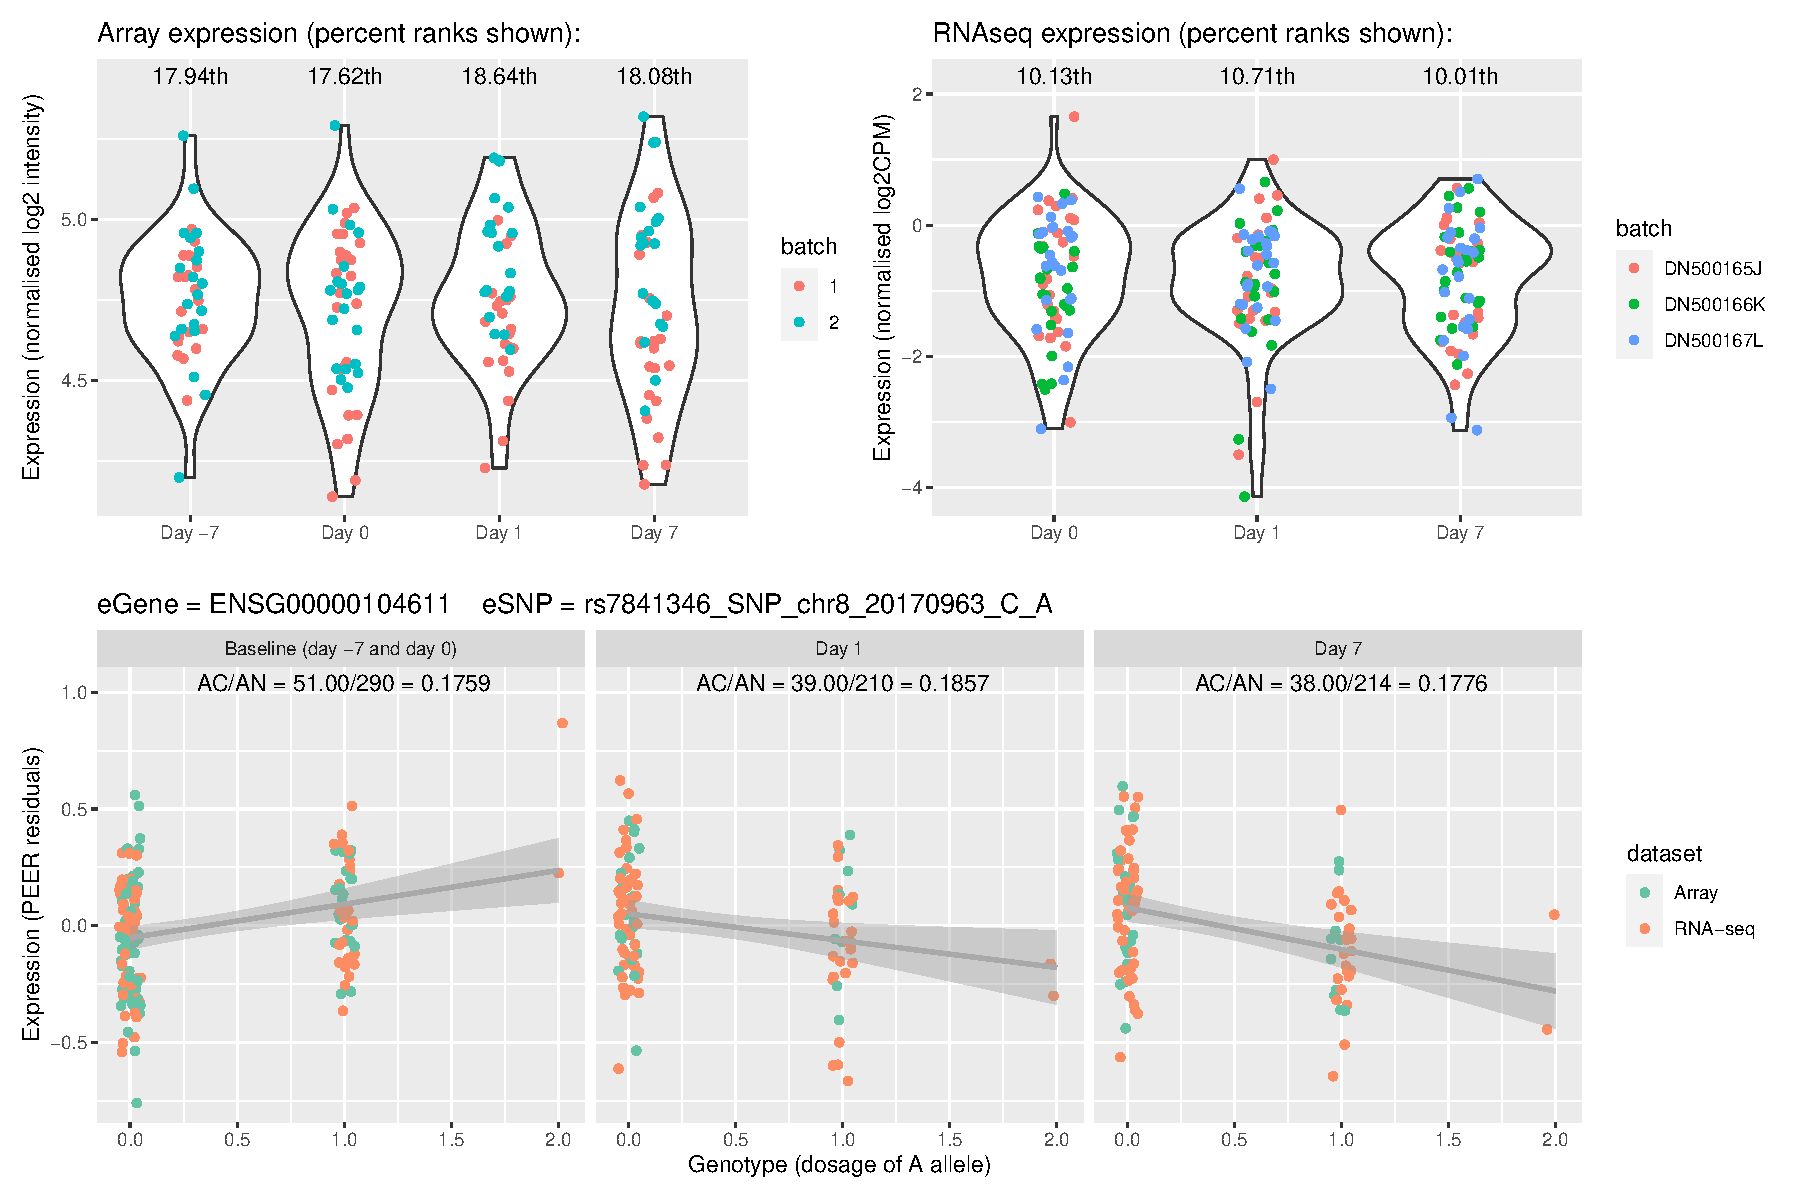
\includegraphics[width=1.0\textwidth,page=1]{mainmatter/figures/chapter_03/plot_dge_eqtl_genotypes.ENSG00000104611,rs7841346_SNP_chr8_20170963_C_A.pdf}
    \caption{\gene{SH2D4A}, strongest reQTL at day 7. Top: Array and \gls{RNAseq} expression before merging with ComBat for mega-analysis. Bottom: eQTL effects at each timepoint condition in the mega-analysis.}
    \label{fig:hird_eQTL_ploteQTL_SH2D4A}
\end{figure}
\todo{convert to subfigures}

\subsection{Genotype by cell type interaction effects}

Given that many \glspl{reQTL} are not explained by differential expression post-vaccination, the presence of cell type-specific \gls{eQTL} effects was considered as an alternate explanation.
As described in \autoref{subsec:hird_reQTL_xCell}, \software{xCell} enrichment scores were used to approximate abundance of seven \gls{PBMC} cell types from the expression data.
After pruning highly correlated cell types to avoid multicollinearity, standardised scores for monocytes, \gls{NK} cells and plasma cells were tested for genotype interactions.
Within-timepoint full \gls{eQTL} models including the genotype main effect, the three cell type abundance main effects, and three cell type-genotype interaction terms, were fit using \software{lme4qtl}, 
then compared to a nested model excluding the three interaction terms.

% TODO: why include the main effect?

\todo{siunitx permits uncertainties}
Significant cell type interactions were detected at 16/1154 \glspl{reQTL} (BH FDR < 0.05) in any timepoint, including \gene{ADCY3} at day 1 ($\chi^2(3) = \num{26.290769}$, \gls{LRT} BH FDR = \num{9.539518e-05}).
Although the genotype effect size was \num{0.255954767} (SE = \num{0.03339378}) in the nested model,
the estimate in the full model was \num{-0.007216815} (\num{0.06656115});
with the three cell type-genotype interaction term estimates being:
monocyte=\num{0.212978154} (\num{0.04897962}),
\gls{NK} cells=\num{-0.009195402} (\num{0.04470412}),
and plasma cells=\num{0.016151511} (\num{0.06632921}).
\todo{gene set enrichment for cell type interacting genes to further validate xCell score usefulness}
The small magnitude of the genotype main effect in the full model vs. the nested model indicates the \gls{eQTL} effect is driven largely by the monocyte score (or a cell type that is highly correlated with monocyte score, see \autoref{fig:hird_xCell_cos2}).
In the case where the monocyte score is zero (representing an average abundance across all samples, as scores are standardised), the effect of increasing genotype dosage on \gene{ADCY3} expression is minimal.
\missingfigure{expression vs monocyte xCell score, colored by genotype, to visually prove the point}

\subsection{TODO Genotype by platform interaction effects}

% pull platform interaction in as a filter
%
% potential problems with mega discussed b4
% - platform fx
% - Using a fixed effect assumes mean diff between rnaseq and array and forces the slope to the average.
% - lme4qtl interactions with bonferroni
- Perhaps using platform specific effects as a filter for reQTLs.
\todo{Need to consider Nikos' comment that there are too many (1069/13570 significant BH FDR) genotype-platform interactions to use mega-analysis. Consider filtering.}

\subsection{TODO Colocalisation of reQTLs with known \textit{in vitro} condition-specific immune eQTLs}

\begin{outline}

\todo{this analysis is incomplete, and is one of the things I would suggest to round off this chapter}

\1 Colocalisation is used to understand the molecular basis of GWAS associations (of a variety of human disease traits) (Giambartolome, 2014)
\1 Here the inverse: coloc is used to understand the biological relevance of observed reQTL by coloc with known immune QTL

% rs916485_SNP_chr2_24859404_T_C
\1 In a 500 Mb window around the lead \gene{ADCY3} variant rs916485, \software{HyPrColoc} to colocalise with existing datasets and fine map.

\1 Day 1 HIRD colocs with BLUEPRINT and Fairfax monocytes (both stim and non stim), but not with Quach or Schmiedel monocytes (\autoref{fig:hird_eQTL_coloc_ADCY3})
\2 Biases from ethnicity-derived differences in LD?
\2 Also, priors need tuning?
% e.g. Assess priors at adcy3, Then coloc all

% fine mapped to 2_24874775_A_G, nearest gene (45,064 bp downstream to canonical TSS): ADCY3 TSS is at 24919839, rev strand
\1 \software{HyPrColoc} fine maps the signal to rs13407913 (credible set size=1, PP = 1), an intronic variant 45064 bp downstream of the TSS.
    \2 note not accurate due to MAF issues

% note in 2019-06-17_team_meeting.pptx, originally was rs10185143
\todo{FYI the IBD/T cell coloc fine maps to chr2:24935139 T C (rs713586) with PP=1}
\todo{add obesity GWAS}

% Assumptions
% multiethnic
% 1 causal per (cluster/trait), untrue in any bulk

\end{outline}

\begin{figure}
    \centering
    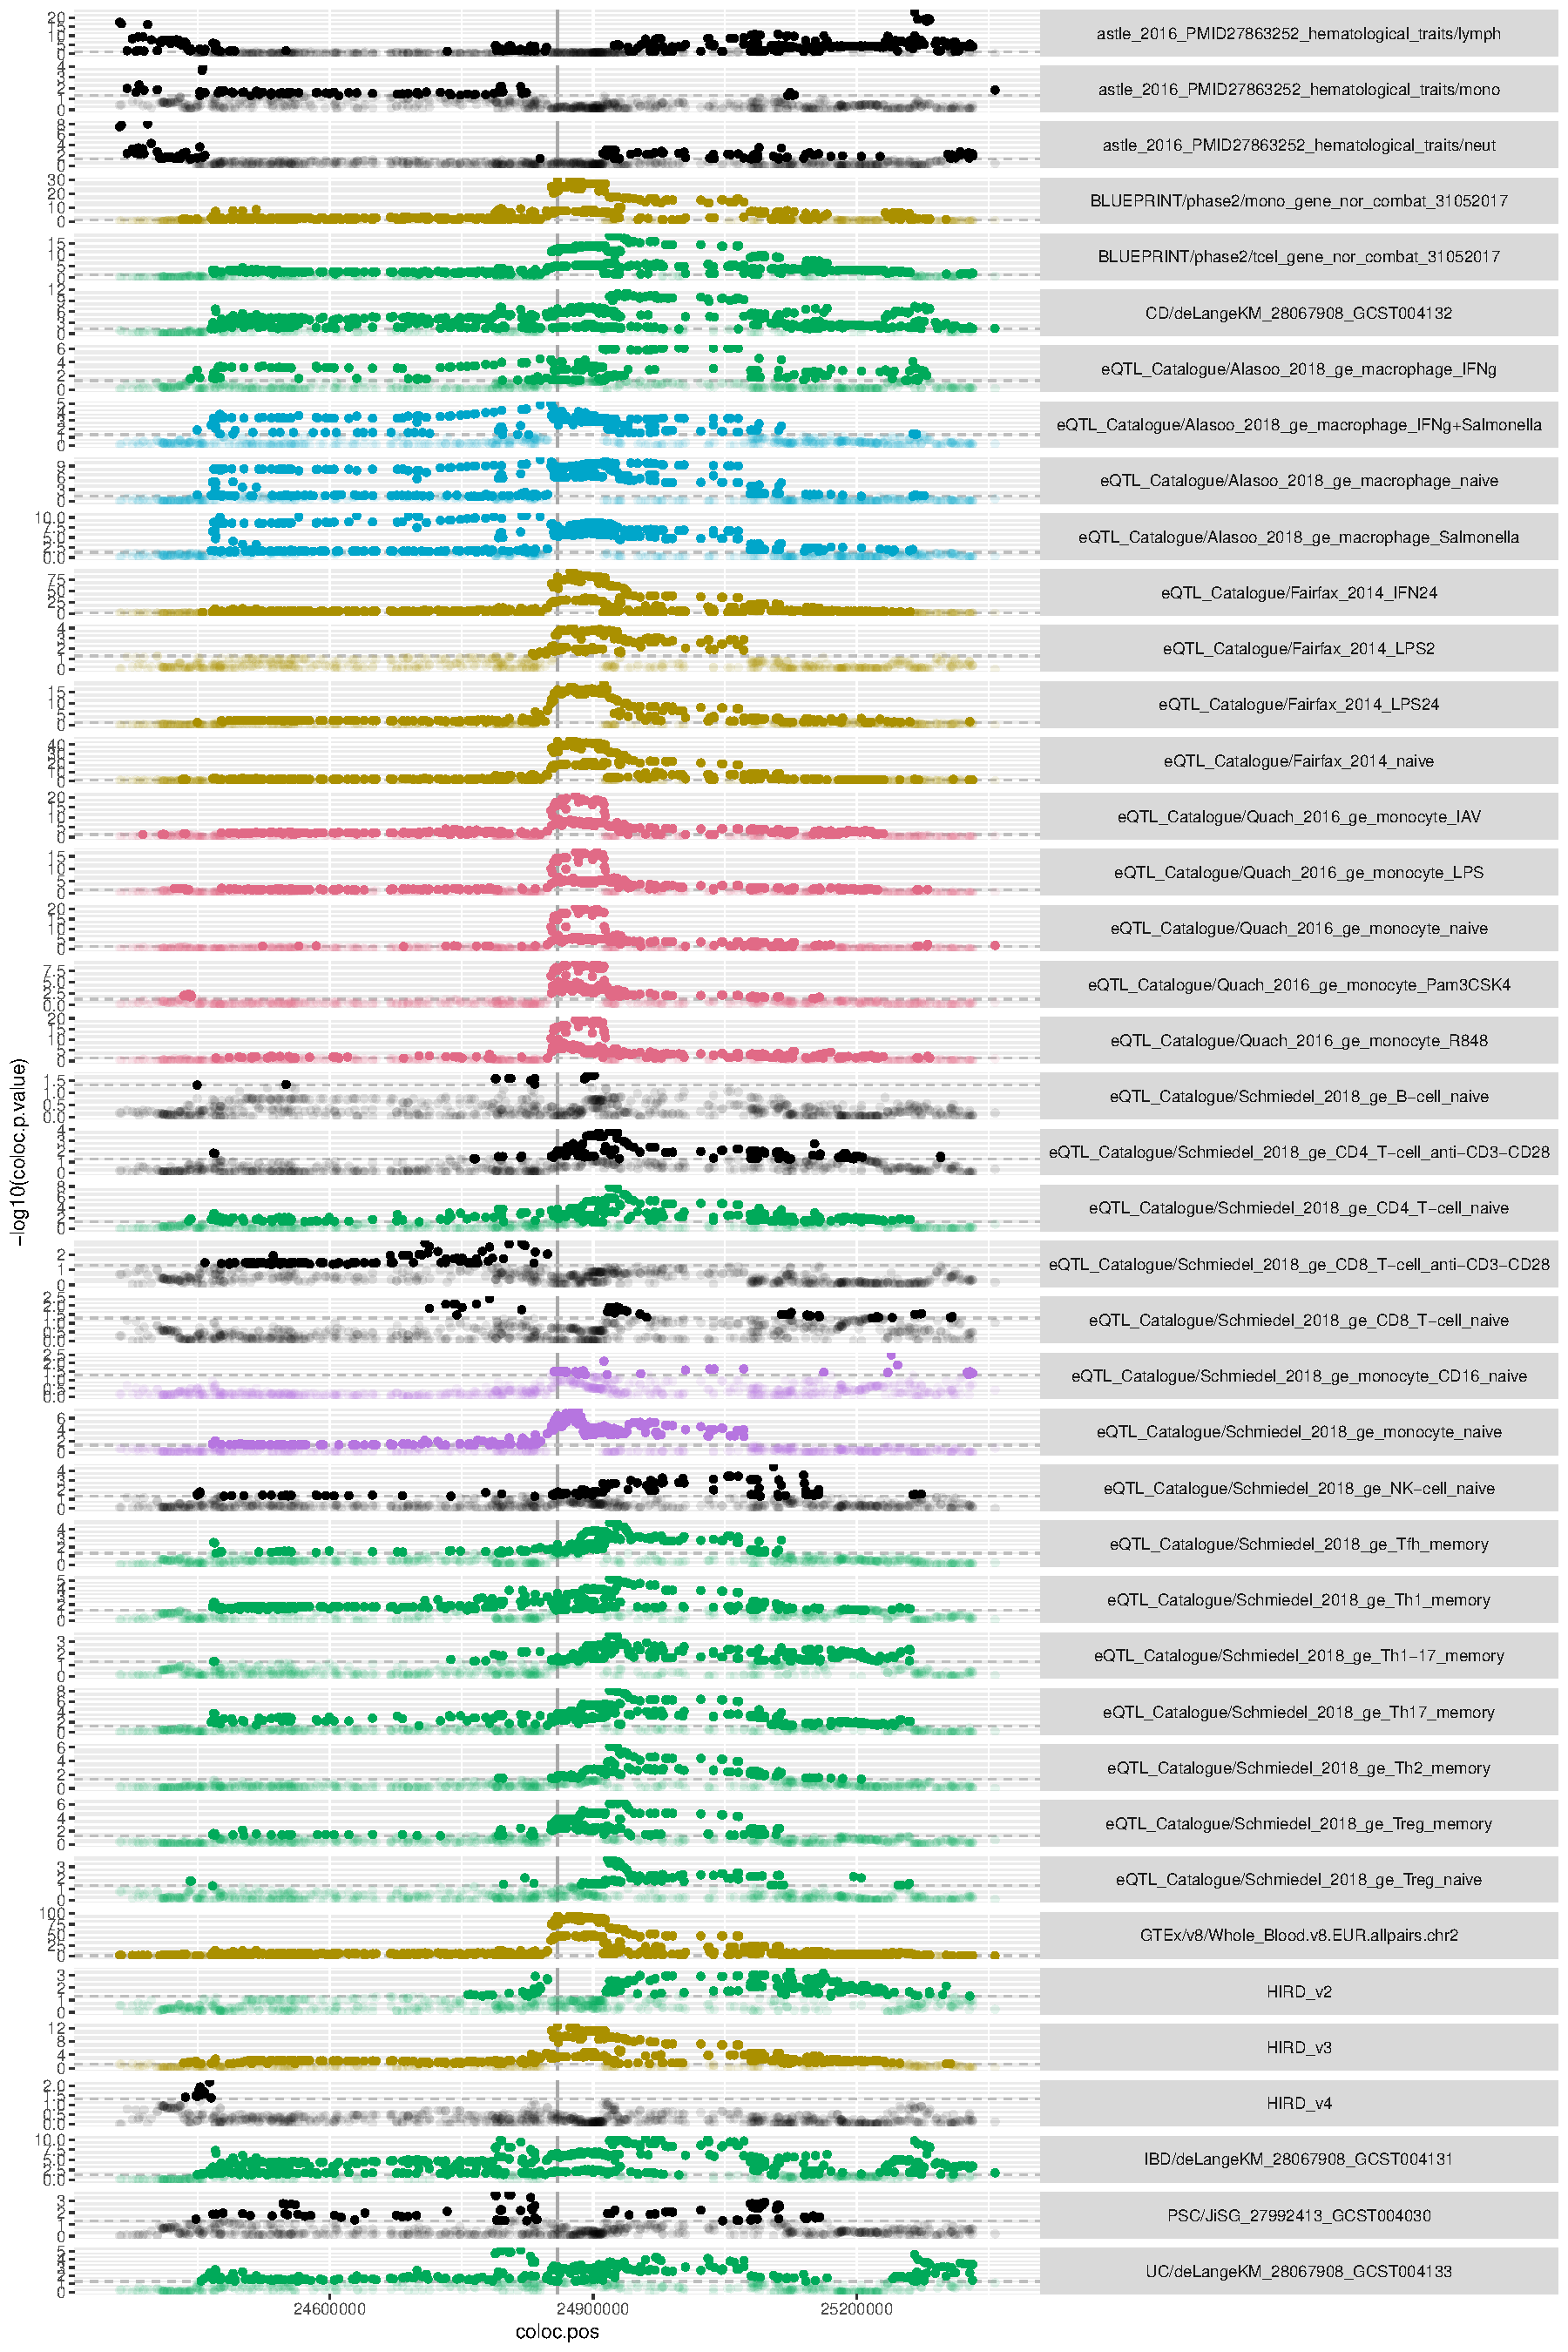
\includegraphics[width=1.0\textwidth,page=1]{mainmatter/figures/chapter_03/perform_coloc.locusPlot.gene_ENSG00000138031.pdf}
    \caption{Multi-trait colocalisation of HIRD reQTL signal at ADCY3 (500 Kb window), with QTL studies from IHEC, BLUEPRINT, eQTL Catalogue, and GWAS Catalogue. Plots are colored by colocalised cluster. Black indicates non-colocalised datasets.}
    \label{fig:hird_eQTL_coloc_ADCY3}
\end{figure}

\section{Discussion}

In the \gls{HIRD} cohort, 
\gls{eQTL} were detected for \percentage{0.5075166} of genes in at least one timepoint, day 0, day 1, or day 7.
% TODO:
% Compare to GTEx
% NOTE: BIOS does not provide full stats
 % You can download the cis-eQTLs detected at a false-discovery rate of 0.05:
% BIOS We detected cis-eQTL effects for 66% of the protein-coding genes and 19% of the noncoding genes tested.
% \todo{\url{https://www.nature.com/articles/ng.3737}, zhernakova2017IdentificationContextdependentExpression, BIOS}
% Each method for determining reQTL has it's own biases.
Even in a joint mapping framework, defining \gls{reQTL} by set significance thresholds, or change in the amount of expression variation explained, will miss classifying equal but opposite effect sizes.
% Other studies have classified effects as magnifying (same sign and greater magnitude) or dampening effects after stimulation\autocite{davenport2018DiscoveringVivoCytokineeQTL},
% but these dampening effects are a mix of same sign and smaller magnitude, and opposite sign effect,
% which may represent distinct molecular mechanisms\autocite{fu2012UnravelingRegulatoryMechanisms}.
I account for the direction and magnitude of effect sizes, defining reQTL strength as the difference in effect size between timepoints.
Most \gls{eQTL} are shared between conditions and replicate well in GTEx whole blood;
\percentage{0.1675621} of lead \gls{eQTL} for each eGene were \gls{reQTL} that differed in effect size between timepoints.
\todo{compare sharing with mashr and ongen2017EstimatingCausalTissues}
% TODO: mashr is less condition specific inclined
% huang2020NeonatalGeneticsGene
% About 10–50% of the condition-specific signals were replicated using a multivariate adaptive shrinkage (mash) model (Supplementary Fig. 3B)20.

% Also see for conditional:
% https://academic.oup.com/hmg/article/26/8/1444/2970473
% https://journals.plos.org/plosgenetics/article?id=10.1371/journal.pgen.1003649
Multiple independent eQTLs are present for a large fraction of eGenes\autocite{zeng2019ComprehensiveMultipleEQTL}.
As the lead variant for reQTL assessment for each eGene was chosen based on significance across all conditions, I can not detect reQTL that are masked by a stronger shared eQTL at that gene.
This is not expected to be uncommon, as the effective sample size for shared eQTLs is usually large due to borrowing of information across conditions.
Secondary \gls{eQTL} signals tend to be weaker, more distal to the TSS, more likely to be enriched in enhancers rather than promoters, and importantly, more context-specific\autocite{vandiedonck2017GeneticAssociationMolecular,dobbyn2018LandscapeConditionalEQTL}.
The proportion of genes with reQTL I detect based on only the lead signal likely represents a lower bound.

% list of other missed:
% low MAF not tagged

Given the larger global changes in expression vs. baseline at day 1 compared to day 7 described in \autoref{ch:hird_DGE}, 
% that these changes are mostly tied to innate immune activation \todo{sectionref},
% and that innate immunity is under stronger genetic control than adaptive immunity\autocite{patin2018NaturalVariationParameters},
the larger number of \glspl{reQTL} detected at day 7 was unexpected (819 vs. 1002).
Opposite sign effects among \gls{reQTL} post-vaccination were common.
% This is methodologically unsurprising, as opposite sign of effect tends to result in greater difference in betas given to the beta-comparison approach.
Prevalance of opposite sign effects between pairs of conditions has been previously described in multi-tissue studies.
In \autocite{mizuno2019BiologicalCharacterizationExpression}, the proportion of opposite sign effects as a percentage of all eGenes was \percentage{0.074} (48 tissues);
in \gls{HIRD}, I find
39/6887 (\percentage{0.005662843}) at day 1,
and 211/6887 (\percentage{0.03063743}) at day 7.
In \autocite{fu2012UnravelingRegulatoryMechanisms}, the proportion of opposite sign effects as percentage of all reQTLs was \percentage{0.044} (5 tissues);
in \gls{HIRD}, I find
39/819 (\percentage{0.04761905}) at day 1,
and 211/1002 (\percentage{0.2105788}) at day 7.
% TODO comment on n tissues
The enrichment of opposite sign effects in \gls{HIRD} is also apparent at day 7.
\todo{I'm not exactly sure why at the moment. Enrichment analyses so far have not turned up much. Up regulation of cell cycle TFs is a possibility.}
The strongest reQTL at day 7 is one such opposite sign effect;
\gene{SH2D4A} has constitutive expression in T cells, B cells, macrophages, and \glspl{DC}, 
encoding a adapter protein involved in intracellular signal transduction\footnote{\url{https://doi.org/10.1111/j.1600-065X.2009.00829.x}}.
An approach for validating these opposite sign \gls{reQTL} using the existing \gls{HIRD} \gls{RNAseq} data is \gls{ASE} (e.g. \autocite{kumasaka2016FinemappingCellularQTLs}),
% \todo{switch to Allele-Specific QTL Fine Mapping with PLASMA}
where one would expect true opposite sign \gls{reQTL} effects would also be recapitulated as opposite directions of expression imbalance.

The strongest \gls{reQTL} detected at day 1 was \gene{ADCY3}, a membrane-bound enzyme that catalyses the conversion of ATP to the second messenger cAMP\autocite{wu2016AdenylateCyclaseNew}.
\Glspl{GWAS} have identified \gene{ADCY3} as a candidate gene for diseases such as obesity\autocite{wu2016AdenylateCyclaseNew} and IBD\autocite{mcgovern2015GeneticsInflammatoryBowel}.
\todo{replace mcgovern2015GeneticsInflammatoryBowel with more recent}
%
\gene{ADCY3} has been identified as a target for reQTLs in multiple studies involving stimulated blood immune cells:
% In fact, six (SLFN5, ARL5B, SPTLC2, IRF5, ADCY3, CCDC146) of the 38 genes
% implicated in our reQTL mapping were also identified in a recent reQTL mapping
% study for Escherichia coli lipopolysaccharide, influenza, and interferon-β in
% dendritic cells [35].
% Aside from \gene{ADCY3}, I also replicate\autocite{caliskan2015HostGeneticVariation} a day 1 reQTL at \gene{SLFN5} (PVE increase from \num{0.27048709} to \num{3.386358e-01}, p diff = \num{4.882379e-02}).
in \gls{PBMC} 24h post-infection with rhinovirus\autocite{caliskan2015HostGeneticVariation},
in whole blood \textit{in vivo} day 1 after vaccination with seasonal \gls{TIV}\autocite{franco2013IntegrativeGenomicAnalysis},
% Examples of three reQTL among genes found only in M. leprae sonicate stimulated
% cells or non-stimulated cells. For each gene ((A) ADCY3, (B) DNAAF1 and (C)
% ZNF517): the left panel corresponds to the expression of the gene in
% non-stimulated cells while the right panel depicts expression of the gene in
% stimulated cells. The gene identity is indicated above each pair of graphs. The
% gene expression level in log2 scale (y-axis) is plotted for each genotype
% (x-axis). Of note, reQTL for the ADCY3 and DNAAF1 genes have been found by
% other studies using distinct pathogens or molecules as stimuli, while the reQTL
% for ZNF517 is a newly identified reQTL [21, 22, 24, 26]. ADCY3 is among the
% most upregulated genes after stimulation with M. leprae antigens and has been
% identified as part of the T1R gene set signature identified by Orlova et al.
% [32]. The reQTL for DNAAF1 displays the strongest p value among the reQTL we
% identified.
and in whole blood after stimulation with \text{M. leprae antigen} for 26-32 h\autocite{manry2017DecipheringGeneticControl}.
Given the diversity of stimulations and tissue types, the effect is likely a consequence of general immune activation, rather than a Pandemrix-specific response.

Statistical colocalisation suggests that the day 1 reQTL signal identified here is likely to be a monocyte-specific effect---and independent to the IBD signal, which colocalises with T cell and macrophage datasets.
The proportion of monocytes in the PBMC increase at day 1, supported by both FACS\autocite{sobolev2016AdjuvantedInfluenzaH1N1Vaccination} measurements, and an increase in monocyte xCell score.
Expression of \gene{ADCY3} is not monocyte-specific, as despite the increase in monocyte proportion, no upregulation is observed at day 1.
\todo{add lfsr.dge}
Colocalisation is also not restricted to stimulated monocytes,
hence the signal could be hypothesised to result simply from the increased proportion of the bulk sample taken up by monocytes,
rather than a upregulation-driven increase in detection power,
or a vaccine-induced activation of the locus at day 1.
\todo{need to consider: if this kind of thing is what bulk in vivo reQTL can find, they what is the additional value over FACS?}
% TODO: need to consider more cell types one by one?

% TODO: do we fall into the Table 2 Fallacy? we should not interpret cell count estiamte params as causal effects, but moderation is demonstrable
% http://www.dagitty.net/learn/graphs/table2-fallacy.html
Changes in relative abundances for many cell types occur in the bulk PBMC samples after vaccination.
I accounted for the effect of abundance on mean expression including xCell scores and PEER factors as fixed effects in the model,
and also considered the effect of abundance on the genotype effect using interaction terms between xCell scores and genotype.
Due to the modest sample size, and computational requirements for \software{lme4qtl}, 
I focused only whether reQTLs that have a detectable main effect may be driven by cell type interactions,
testing only for interactions at significant lead \gls{reQTL},
%
Compared to FACS measurements in a cohort subset, the xCell scores used above were only weakly correlated.
Some discrepancy is expected, as the cell types as defined in the xCell signatures do not directly correspond to the combinations of surface markers used for FACS.
The FACS gating strategy also meant that for some cell populations, the only available FACS measure was a proportion of the previously gated population,
whereas xCell attempts to estimate scores that represent proportions of the whole mixture.
The accuracy of the built-in signatures is lower when applied to the expression matrix for a stimulated state,
likely because the enrichment-based method can not distinguish differential expression of signature genes due to stimulation from actual changes in cell abundance.
% A custom signature matrix can be used for xCell, but this would need to be drawn from an independent study under the same stimulation conditions as \gls{HIRD}, and would not solve the issue of coupled DE and cell abundance.
Nevertheless, as assuming a single genotype where cell-type specific slopes are likely is inappropriate, so xCell scores were used as a best approximation.
%
At 16/1154 reQTLs, the genotype effect was detected to interact with abundance of one or more of the tested cell types (or a correlated cell type).
At the day 1 \gene{ADCY3} reQTL, the genetic effect can be mainly attributed to the monocyte score-genotype interaction term, further supporting the hypothesis that it is monocyte-specific.

% TODO: Franco replication
% 20 genes from Franco
% 12/17 DGE replicated
% 14/17 eGenes replicated, none were reQTL
\todo{dge is coupled to reqtl, if you do an enrichment of dge+reqtl overlap genes, likely their enrichment is driven by DGE signal}

A pressing question remains: what molecular mechanisms underlie the \gene{ADCY3} \gls{reQTL}, and indeed the remainder of the \glspl{reQTL}?
Power differences due to condition-specific expression are unlikely to explain a large proportion of reQTLs.
As in \autocite{kim-hellmuth2017GeneticRegulatoryEffects, davenport2018DiscoveringVivoCytokineeQTL}, the overlap between differentially expressed genes and genes with reQTL was poor,
and reQTL were not more likely to be differentially expressed compared to genes without reQTL.
%
% TODO
% reqtl already tests whether change in e is diff by g, so no need to check DGE too
% may be no reason to believe that most DGE is also the most reQTL
One mechanism by which cis-eQTL affect expression is through their impact on \gls{TF} binding affinity to motifs in promoters and enhancers\autocite{pai2015GeneticMechanisticBasis}.
Immune cells, including monocytes, are regulated by cell type specific \glspl{TF}\autocite{choudhury2016IdentifyingCellTypeSpecific}.
\todo{harmonise terminology for 'opposite'}
Cell type specific expression of different \glspl{TF} have been proposed as a model for explaining magnifying, dampening and opposite reQTL effects;
\todo{ check "rs2223286 is associated with profound directional effects in the expression of SELL dependent upon genotype, with the minor C allele associated with increased expression of SELL in B-cells and reduced expression of SELL in monocytes " }
for example, opposite effects can result from \glspl{TF} regulating the same gene, that are activating in one cell type and suppressive in another\autocite{fu2012UnravelingRegulatoryMechanisms}.
There is evidence that \gls{TF} activity is important for \textit{in vivo} immune reQTL:
\autocite{caliskan2015HostGeneticVariation} found rhinovirus reQTLs in \glspl{PBMC} were enriched in ENCODE ChIP-seq peaks for the \glspl{TF} \gene{STAT1} and \gene{STAT2},
and \autocite{davenport2018DiscoveringVivoCytokineeQTL} found interferon and anti-IL6 drug reQTLs likely disrupt \gene{ISRE} and \gene{IRF4} binding motifs.
Rather than condition-specific expression of the eGene, what may be condition-specific is the expression of \glspl{TF} whose activity is affected by the reQTL%
\footnote{
    A cursory scan of \gls{TF} motifs disrupted by the location of the fine-mapped \gene{ADCY3} reQTL intronic variant rs13407913 on \url{https://ccg.epfl.ch/snp2tfbs/snpviewer.php},
    does indeed show several motifs (for NR2C2, HNF4A, HNF4G, NR2F1)
    where the PWM score is higher for the ALT allele, 
    consistent with the direction of effect for the day 1 reQTL.
}.
% introns can be TF bound https://journals.plos.org/plosone/article?id=10.1371/journal.pone.0046784
% http://54.245.180.226/php_file/multiple.php?ID=rs13407913
% SP1 is monocyte specific https://europepmc.org/article/med/28008225
% and upreg at d1

Finally, I address the prospect that common genetic variation may explain some variation in antibody response to Pandemrix.
% TODO
% Based on studies in twins, genetics seems to contribute only marginally to this heterogeneity
% in vaccination outcomes in adults, suggesting environmental factors as key drivers [19,20].
% tsang2020
I have indirectly demonstrated genotype-dependent effects on expression response by identifying reQTLs with differing effect size between timepoints,
but have not yet to determined resulting genotype-dependent differences in antibody phenotypes.
Some of the identified reQTLs will undoubtedly affect genes whose expression or post-vaccination expression change correlates with antibody response, 
but correlation is not transitive\autocite{langford2001PropertyBeingPositively},
\todo{note coloc doesn't distinguish pleiotropy from mediation?}
% many many scenarios possible: https://genomemedicine.biomedcentral.com/articles/10.1186/s13073-019-0613-2/figures/1
and a formal tests such as the \gls{CIT}\autocite{millstein2009DisentanglingMolecularRelationships} are required to distinguish mediation of genotype-antibody associations through gene expression from competing models.
\autocite{franco2013IntegrativeGenomicAnalysis} realised this, but concluded that they had insufficient power with a greater sample size and comparable study design to \gls{HIRD}.
The \gls{HIRD} cohort is also too small for a direct \gls{GWAS} of Pandemrix antibody response.
% TODO: after all that Intro about gwas to function, we unfortunately lack the gwas part here
% https://stats.stackexchange.com/questions/176384/do-underpowered-studies-have-increased-likelihood-of-false-positives
% The basic problem with underpowered studies is that, although the rate of false positives (type I error) in hypothesis tests is fixed, the rate of true positives (power) goes down. Hence, a positive (= significant) result is less likely to be a true positive in an underpowered study. This idea is expressed in the false discovery rate [2], see also [3]. This seems what the quote refers to.
% An additional issue often named regarding underpowered studies is that they lead to overestimated effect sizes. The reasons is that a) with lower power, your estimates of the true effects will become more variable (stochastic) around their true value, and b) only the strongest of those effects will pass the significance filter when the power is low. One should add though that this is a reporting problem that could easily be fixed by discussing and reporting all and not only significant effects.
A suitable approach for prioritising reQTL that contribute to the antibody response to Pandemrix will be to leverage external genetic associations to similar phenotypes,
for example, colocalisation with existing GWAS summary statistics for antibody response to a similar type of adjuvanted, inactivated vaccine.

% TODO: need ASE, 
% not just for validation of the effect, but because eqtl effect size is less than intepretable, and stratified analysis tends to use different adjusted effects per condition.
% TODO:
% is ASE affected by cell comp?

\todo{add 1 concluding line}
\todo{Overall I feel like the chapter is too descriptive, and falls short of making biological insights into Pandemrix response. Any additional analyses would hope to address that.}

% TODO: add a whilst we were not able to X in the intro, the field has advanced by Y, future Z needed

% TODO
% Would like to know what cell types for all reqtl, but limited by a trying one by one strategy
% Always might miss one not tried
% Not viable for scaling
% SC rnaseq

% TODO are these reQTL interesting?

% TODO
% Would like to know what cell types for all reqtl, but limited by a trying one by one strategy
% Always might miss one not tried
% Not viable for scaling
% SC rnaseq
